\documentclass{my_paper}
\usepackage{ctex}
\usepackage[textwidth=444bp,vmargin=2.5cm]{geometry}
\usepackage{array}
\usepackage{float}
\usepackage[dvipsnames]{xcolor}
\usepackage{graphicx}
\usepackage{booktabs}
\usepackage{epstopdf}
\usepackage{enumitem}
\usepackage{multirow}
\usepackage{amsmath}
\usepackage{subcaption}
\usepackage[T1]{fontenc}    
\usepackage{newtxtext, newtxmath}  
\usepackage{caption}
\usepackage[dvipsnames]{xcolor}
\usepackage{listings}
\usepackage{xcolor}
\usepackage{listings}
\usepackage{xcolor}
\lstset{
    language=Python,
    numbers=left,
    numberstyle=\tiny,
    keywordstyle=\color{blue},
    commentstyle=\color{gray},
    stringstyle=\color{red},
    basicstyle=\ttfamily
}
\begin{document}
\newpage
\begin{center}
\lunwenbiaoti \\
%---------------------------------------摘要------------------------------------
\vspace{2ex}
\zhaiyao
\end{center}

蔬菜类商品保鲜期较短,因而商超会根据历史销量和需求情况每天进行补货。本文基于单目标规划,采用基于利润权重的蔬菜定价算法建立了蔬菜品类和单品的定价补货决策模型,并通过基于动态权重的离散化贪心和基于分支限界的0-1背包问题等动态规划算法,为商超决策蔬菜类商品的自动定价与补货提供建议。\par
首先对附件数据进行预处理,对缺失值、异常值进行清洗,分析各附件数据关联,合并数据集和分析数据性质后最终确定使用\textbf{完全成本加成定价}进行分析。\par 
针对蔬菜及单品销售量分布规律及相互关系分析的问题,首先通过绘制折线图与分析数据特征,得到蔬菜销售量具有\textbf{季节性}、\textbf{突变性}、\textbf{贝塔分布和非正态性}的特点。再通过协方差矩阵定量分析得出不同品类之间蔬菜销售量的相关性。为进一步分析品类间销量关系,采用\textbf{VAR向量模型}验证,证明了结果的合理性。对品类内的各单品,绘制相关系数热力图,得出同品类的不同品种间通常存在负相关性,即\textbf{相互替代}的关系。\par
针对蔬菜品类日补货量和定价决策的问题,首先以品类为单位计算单品利润占比,进而计算出各品类的成本加成定价,并对计算结果进行\textbf{正态性检验},将其与品类销售量进行\textbf{相关性分析},计算$Spearman$相关系数,从而得出某一品类的销售量与成本加成定价间呈\textbf{负相关},故后续求解时考虑成本加成利润率对销售量的影响。考虑到品类销售量符合贝塔分布,需要分析季节性对其影响,因而采用\textbf{SARIMA模型}预测各品类7月1日-7日的补货量作为后续求解的基准,计算得模型拟合优度高,证明预测结果合理。对于未来一周的补货总量和定价策略求解,以成本加成利润率$r_i$为决策变量,商超的利润为规划目标,采用\textbf{基于动态权重的离散化贪心和动态规划算法}解决最大利润问题。最终确定了各品类蔬菜的补货定价策略,此时商超一周收益最大。\par
对于7月1日的单品补货和定价决策问题,首先对蔬菜单品基于6月24日-30日补货量大于0和利润率占比大于1\%,选出合适单品\textbf{49种}。因相关数据量较少,从而选用\textbf{GM(2,1)模型}对各单品7月1日的销售数据进行预测,并对预测结果进行分析,证明其合理性。然后基于预测的销售数据,针对是否选取某种单品,将7月1日的补货量和定价策略求解转化为\textbf{0-1背包问题},采用基于分支限界的0-1背包动态规划算法处理,计算得到应选择包括云南生菜、小米椒(份)在内的29种蔬菜,此时商超单日理论收益最大。\par
对于优化补货和定价决策的问题,本文分析蔬菜新鲜度变化、消费者喜好程度和仓储成本等因素对商超收益的影响,考虑蔬菜新鲜度变化时,依据附件中扫码销售时间推断出商超开放时间,并划分蔬菜的新鲜度,建立\textbf{基于新鲜度的蔬菜售价公式};考虑消费者喜好程度时,消费者对于不同新鲜度的蔬菜喜好程度相异,依据蔬菜新鲜度的分界点,给出消费者的\textbf{指数偏好函数};考虑仓储成本时,因需要人工取货、人工卸货、人工装货等操作,因而总体成本会上涨一定比例。再通过计算机模拟的方式,分析各类因素的引入对于商超收益的影响。

\begin{guanjianci}
 \quad \textbf{完全成本加成定价}\textbf{相关性分析}\quad \textbf{利润权重的加成定价}\quad \textbf{SARIMA模型}\quad \textbf{动态规划}
\end{guanjianci}

%----------- 正文 ----------





% \newpage

%----------- 一、问题重述 ----------
\newpage
\section{一、问题重述}
\subsection{问题背景}
生鲜商超中蔬菜类商品保鲜期通常较短,且其品相和价值随销售时间的延长而不断变差,使得当日不新鲜蔬菜需打折销售,隔日蔬菜无法再售。下表是部分大型商超的调价频率\cite{我国超市优质生鲜蔬菜动态定价问题研究}
\begin{table}[H]
    \centering
    \caption{部分大型商超调价频率表}
    \begin{tabular}{ccccc}
        \hline & 超市发 & 乐天玛特 & 华联 & 沃尔玛 \\
        \hline 促销方式 & 
        $\begin{array}{l}\text { 每天都有特价和让 } 
        \text {  } \\
        \text { 利普通蔬菜 }\end{array}$ &
         $\begin{array}{l}\text {有}
        \text {特价普通蔬}
        \text {菜}\end{array}$ &
         $\begin{array}{l}\text {有} 
        \text {特价普通蔬菜} \\
        \end{array}$ & 
        $\begin{array}{l}\text {普}
        \text {通蔬菜有特价} \end{array}$ \\
        调价频率  & 三次/每日 & 一次/每日 & 一次/每日 & 两次/每日 \\
        \hline
        \end{tabular}
    \label{商超调价频率}
\end{table}
由表\ref{商超调价频率}可知,商超每天需要根据产品的新鲜情况,一次或多次地给部分商品打折销售。同时鉴于商超所销售的蔬菜品类众多、产地不尽相同与进货时间较早,故商家每天需根据蔬菜品类做出补货决策。\par
此外,由于蔬菜通常由销售者决定价格的主导权,所以蔬菜的定价一般采用成本加成定价的方法\cite{wang2003},即商超常对运损和品相变差的商品采取打折销售的措施,以谋求商超整体收益最大化。同时由于商超销售空间存在限制,所以对蔬菜类商品的市场需求进行可靠分析,并设置合理的蔬菜销售组合变得十分重要。
\subsection{问题要求}
在已知某经销商经销的$6$个蔬菜品类的商品信息,和了解这些商品的流水情况明细和批发价格的情况下,基于已有数据进行分析建模,解决以下几个问题:
\begin{enumerate}
    \item 根据相关附件,分析不同品类蔬菜类商品或不同蔬菜单品之间可能存在的关联关系,并给出蔬菜各品类及单品销售量的分布规律及相互关系。
    \item 以品类为单位,分析各蔬菜类的销售总量和成本加成定价的关系,并给出各蔬菜品类未来一周(2023.7.1起)的补货策略和定价策略,使得商超收益最大。
    \item 进一步制定有关蔬菜单品的补货计划,在控制可售单品总数,订购量满足最少陈列要求的要求下,基于$(2023.7.1)$这一天前一周的可售品种,给出当日的单品补货量和定价策略,并在满足市场对各品类蔬菜商品需求的前提下使得商超收益最大。
    \item 给出进一步优化蔬菜商品的补货和定价决策模型所需要的数据,给出收集此类数据的理由,分析该类数据对商超收益和蔬菜补货的影响。
\end{enumerate}
%----------- 二、问题分析 ----------
\section{二、问题分析}

\subsection{问题一的分析}
针对第一小问,要求分析不同品类蔬菜和不同蔬菜品种的销售量分布规律,由于蔬菜的销售量均为定量变量,且据题知销售量与时间存在关联关系,故本文分别从描述性统计的角度和统计规律的角度,分析各品类蔬菜和各种蔬菜的销售量的分布规律。\par
针对第二小问,首先通过协方差矩阵和相关系数定性地分析不同种类蔬菜的相互关系,接着采用向量自回归模型定量分析各个蔬菜品类之间的动态相互作用关系,二者彼此验证共同阐述相互关系;对于各种蔬菜单品相互关系的分析,我们同样采取协方差矩阵和相关系数结合的方式定性分析。
\subsection{问题二的分析}
针对第一小问,首先以加权的方式计算得出各品类蔬菜的总成本加权定价,再与各品类蔬菜的补货量即销售量进行相关性分析,分析其关系。\par
针对第二小问,根据数据的时序特征,采用SARIMA模型对各蔬菜品类未来一周的日补货总量进行预测,并根据模型质量分析该预测较为准确。\par
针对第三小问,通过先前得到的总成本加权定价计算出各品类的成本加成利润系数,再通过三次样条插值拟合出销售量与成本加成定价的定量关系,进而得出利润系数与销售量的关系。以利润系数为决策变量,商超利润的最大值为优化目标,使用离散化贪心动态规划算法进行优化求解。

\subsection{问题三的分析}
针对第一小问,首先根据题意对相关数据进行筛选,剔除与本问无关的数据。然后采用GM(2,1)模型对各单品在2023年7月1日的相关数据进行预测。\par
针对第二小问,首先引入0-1变量表征某单品是否被选中,接下来以商超收益为优化目标,以为决策变量,使用基于分支限界的0-1背包动态规划进行优化求解。
\subsection{问题四的分析}
针对题目要求,新引入蔬菜商品新鲜度\cite{gu2023},消费者的消费心理和消费需求,以及蔬菜商品库存成本进行单独和共同分析,分析各因素单独附加和彼此搭配对商超收益的影响情况。\par
基于上述分析与描述,给出本文所构建的模型结构框架图如图\ref{模型结构框架图}所示:
\begin{figure}[H]
 \centering
 \includegraphics[width=\textwidth]{模型结构框架图.png} %1.png是图片文件的相对路径
 \caption{模型结构框架示意图} %caption是图片的标题
 \label{模型结构框架图} %此处的label相当于一个图片的专属标志,目的是方便上下文的引用
\end{figure}\par
%----------- 三、模型假设 ----------
\section{三、模型假设}
为了便于分析蔬菜类商品的关联关系,并为商超给出恰当的定价与补货策略,本文做出以下假设:
\noindent\par
$\bullet$ 假设本文四份附件所给数据没有误差且真实;\par
$\bullet$ 假设蔬菜退货后不再重新出售,视作额外成本;\par
$\bullet$ 假设每日仅出售当日进货的蔬菜;\par
$\bullet$ 假设不同供应来源的蔬菜视作不同种蔬菜,单品品种由单品编码唯一确定;\par
$\bullet$ 假设每日仅补货一次,且顾客购买量不会超出库存量;\par
$\bullet$ 假设补货量等于销售量加上损失量 ;\par
$\bullet$ 假设蔬菜销售量随时间变化是连续的;\par

%----------- 四、符号说明 ----------
\section{四、符号说明}

\begin{table}[H]
    \centering
    \begin{tabular}{p{2.0cm}<{\centering}p{9.0cm}<{\centering}p{2.0cm}<{\centering}}
    \toprule
    符号 & 说明  \\ 
    \midrule
    $P_i$&     第i种商品最终定价\\
    $C_i$&     第i种商品完全成本\\
    $r_i$&     第i种商品成本加成定价的利润率\\
    $w_{it}$    &周内第i种蔬菜第t天对该品类成本加成定价的权重\\
    $logL$&     对数似然函数值  \\
    $SC$&     贝叶斯信息准则   \\
    $X_i$&   六类蔬菜中第i类蔬菜的销售量 \\
    $X_i^j$& 六类蔬菜中第i类蔬菜的第j阶滞后值 \\
    $W$ & 商超总利润 \\
    $M_i$ & 第i种商品的销售总量 \\
    $S_p(i)$ & 第i种单品占用销售空间 \\
    $t_f$& 商品新鲜度转变时间节点 \\
    $t_i$& 商品销售周期内某一时间点 \\
    $S_i$& 某一时间点的折扣\\
    $m(t)$& 消费者随时间变化的偏好函数 \\
    $s$& 商超服务水平因子 \\
    $f$& 新鲜度变化因子 \\
    $\theta$& 商品新鲜度表征量 \\
    $\lambda$& 商品价值损耗率 \\
    $k_i$& 某一时间点新鲜度影响因子\\
    $h$& 单位仓储成本\\
    \bottomrule
    \end{tabular}
\end{table}
%----------- 五、模型准备 ----------
\section{五、模型准备}
在对各个问题进行建模求解之前,首先对附件中的数据进行相应处理。本题中模型准备主要包括4个方面:数据的清洗,数据的处理,数据集合并与成本加成定价计算。模型准备的示意图如下所示:
\begin{figure}[H]
 \centering
 \includegraphics[width=\textwidth]{模型准备示意图.png} %1.png是图片文件的相对路径
 \caption{模型准备示意图} %caption是图片的标题
 \label{模型准备示意图} %此处的label相当于一个图片的专属标志,目的是方便上下文的引用
\end{figure}\par
\subsection{数据清洗}
首先对附件中数据进行清洗,包括了空缺数据的补全和异常数据的识别和分析。\par
\begin{itemize}
    \item 经过对附件2的处理,我们发现在2020年7月1日至2023年6月30日的1095天中共有10天无销售数据,则为后续分析便利,将此10天内所有蔬菜单品的销售数据均补0,以完善附件2。
    \item 经过对附件3的处理,我们发现在上述1095天中共4天无进货价格数据,且同时这四天也无销售数据,则为简化分析本文中对这四日补货和收益的相关数据不进行相关讨论。
\end{itemize}
\subsection{数据处理}
由附件可知,题目相关数据量较为庞大且类别繁多,为了简化分析难度,共进行了以下操作:
\begin{itemize}
    \item 对于附件1中部分单品名称包含的数字编号,将其视作不同单品蔬菜的一种标识;
    \item 对于附件2中销售类型列,将销售类型为退货的相关数据进行处理。用该种蔬菜当日销售量减去退货量,视作其真实销售量;
    \item 基于附件4中的损耗率,结合附件2计算得到的真实销售量,计算得出各商品的补货量。
\end{itemize}
\subsection{数据集合并}
为了后续数据如成本加成定价等计算处理方便,且由附件可知四则附件均以单品编码作为各单品的标识,因而可以将单品编码作为合并索引,把四个附件内容整合至一个数据表中,从而便于后续分析讨论。
\subsection{成本加成定价分析}
由题可知,蔬菜的定价常采用成品加成定价的方法,即商超对于运损和品相变差的商品会进行打折销售以便谋求更高收益。为后续处理方便,故本文先根据相关公式和所给附件,计算各产品的产品加成定价。\par
成品加成定价法是基于成本来确定商品销售价格的方法,分为完全成本加成定价法和变动成本加成定价法。对于本题来说,因为蔬菜的保质期较短,隔夜蔬菜难以再售,且运输和冷藏蔬菜对于商家均有一定开销,因此采用完全成本加成定价法可以保证每次销售均覆盖了商品的成本,且考虑了额外的固定和变动成本,因此本文采取的是完全成本加成定价法。\par
根据完全成本加成定价法的相关公式\textbf{引用网站},
\begin{equation}
    \label{完全成本加成定价}
    P_i = C_i * ( 1 + r_i )
\end{equation}
\hspace{2em}其中$P_i$代表第i种商品最终定价,$C_i$代表第i种商品的完全成本,本题中包括了进价成本、运输成本和冷藏成本等,$r_i$代表成本加成定价的利润率,即商超根据自身收益需求,从而确定的目标利润率。\par
就本题而言,计算各商品的完全成本加成定价可采取以下步骤:
\begin{itemize}
    \item 完全成本即进货价加上动态成本,即$ C_i = C_{fixed} + C_{loss} $,其中$C_{fixed}$为商品的固定成本,在本题中表征进货成本,$C_{loss}$为商品的损耗成本,在本题中表征运输损耗、退货损耗等等,二者相加即可计算得各单品每日的单位总成本;
    \item 加成率即利润加成除以完全成本,其中利润加成为售价减去完全成本,因而为满足收益需要,商超可以调控售价以改变收益率;
    \item 商品的完全成本加成定价即可根据公式\ref{完全成本加成定价} 计算。
\end{itemize}
%----------- 六、模型的建立与求解 ----------
\section{六、模型的建立与求解}


\subsection{问题一模型的建立与求解}
\subsubsection{各类蔬菜及单品销售量分布规律}
\textbf{Part1: 各类蔬菜销售量分析}\par
由问题一分析,本题需讨论蔬菜各品类及单品销售量的分布规律及相互关系,本文首先对各类蔬菜日销售量情况,绘制了折线图如图\ref{各类蔬菜日销售量}和图\ref{六类蔬菜日销售量}所示:
\begin{figure}[H]
 \centering
 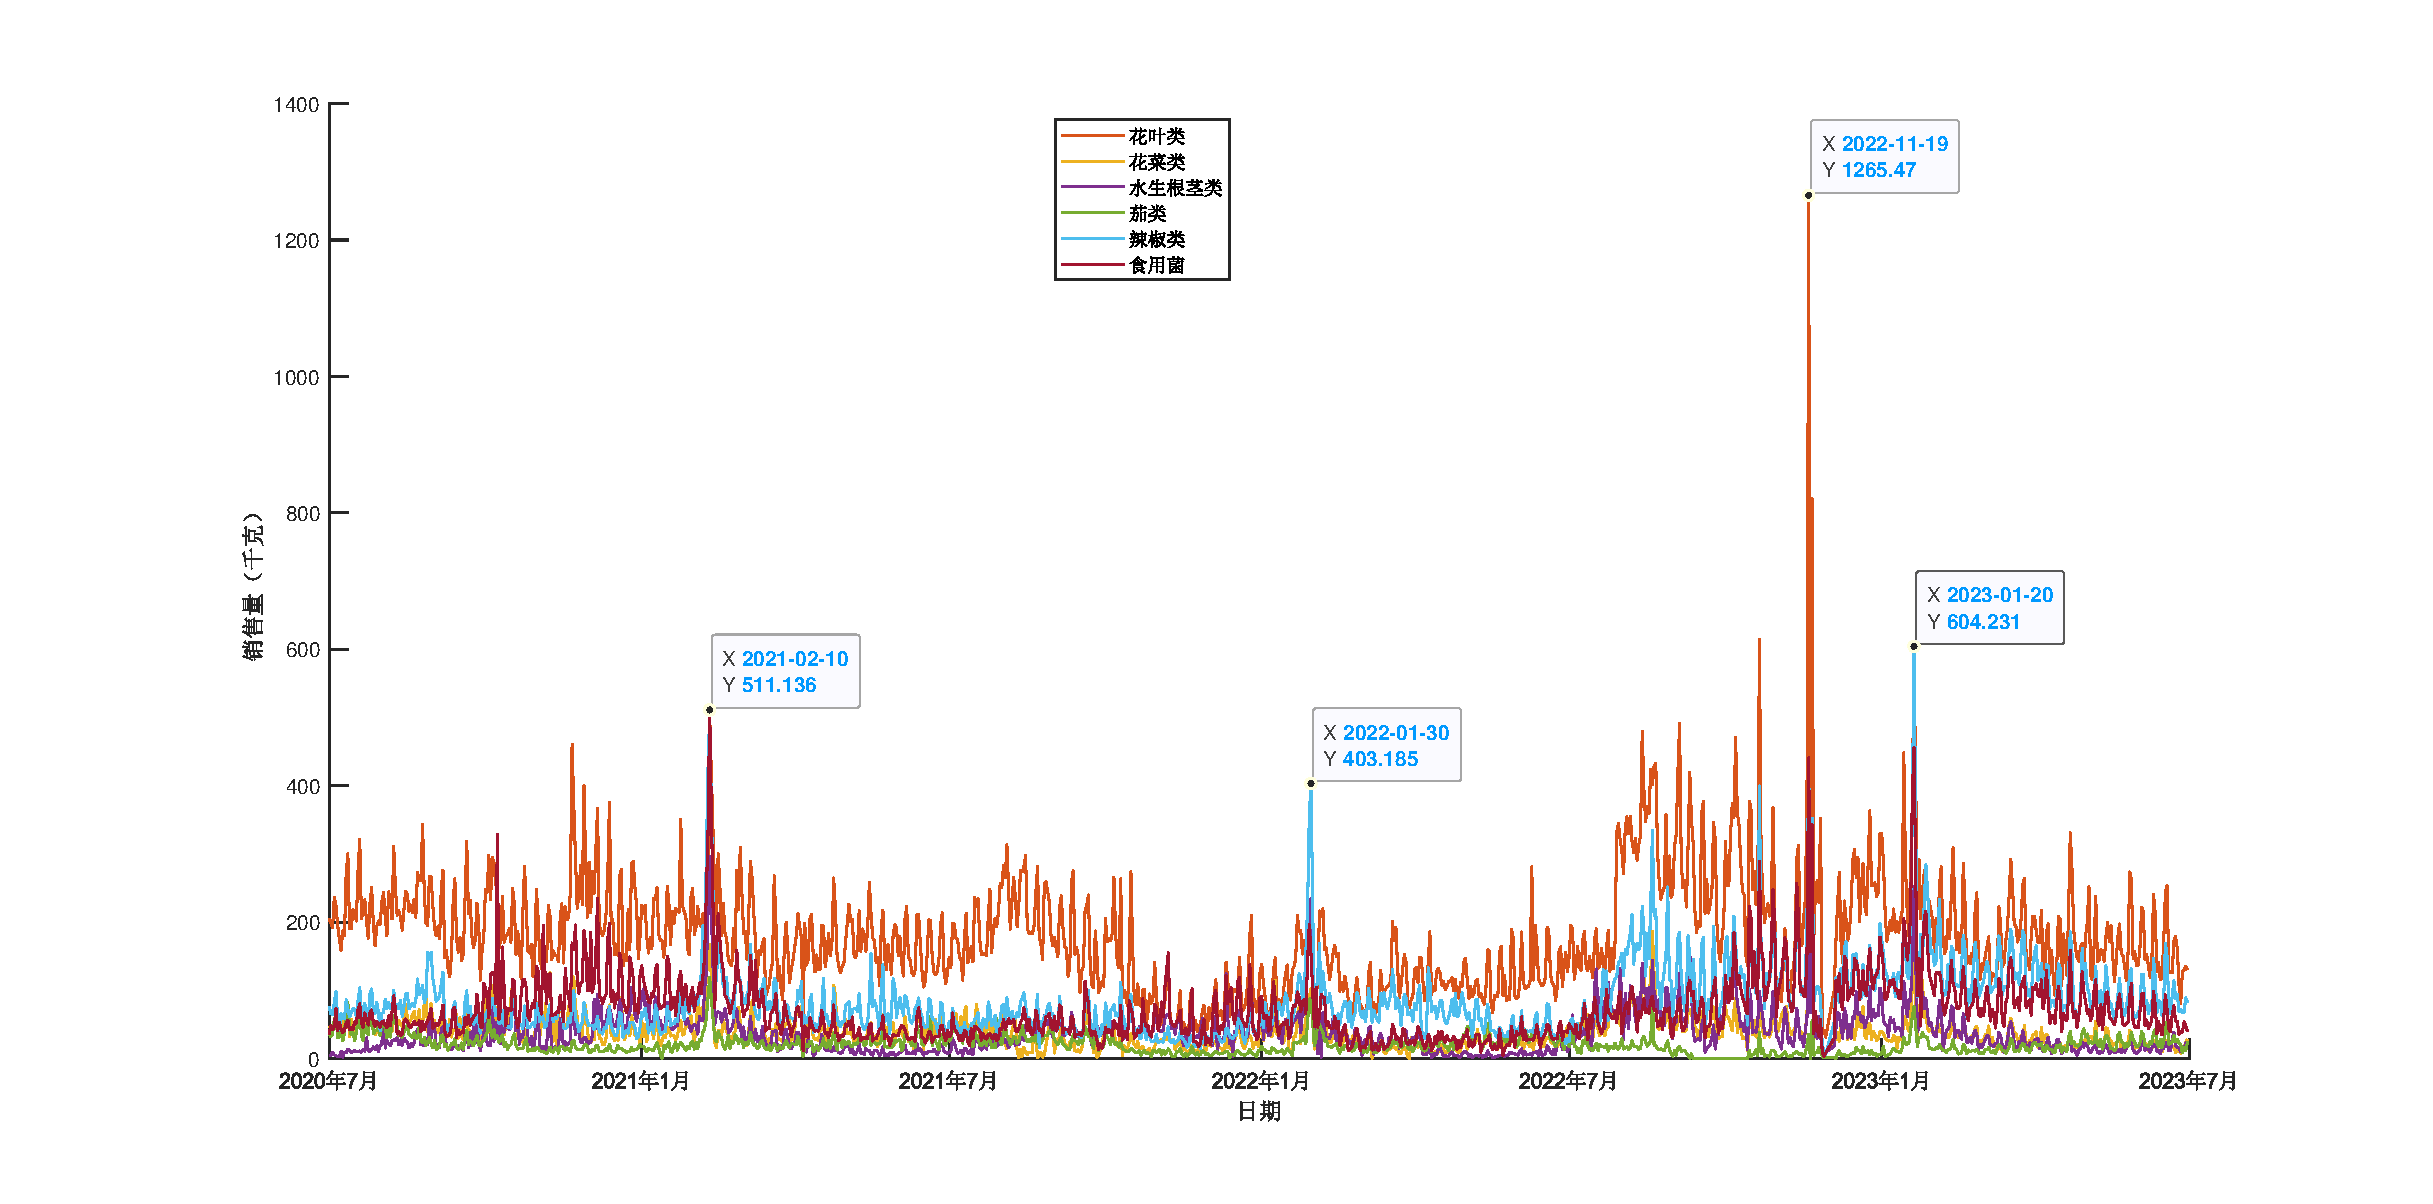
\includegraphics[width=\textwidth]{各蔬菜类日销售量.eps} %1.png是图片文件的相对路径
 \caption{各类蔬菜日销售量} %caption是图片的标题
 \label{各类蔬菜日销售量} %此处的label相当于一个图片的专属标志,目的是方便上下文的引用
\end{figure}\par

\begin{figure}[H]
 \centering
 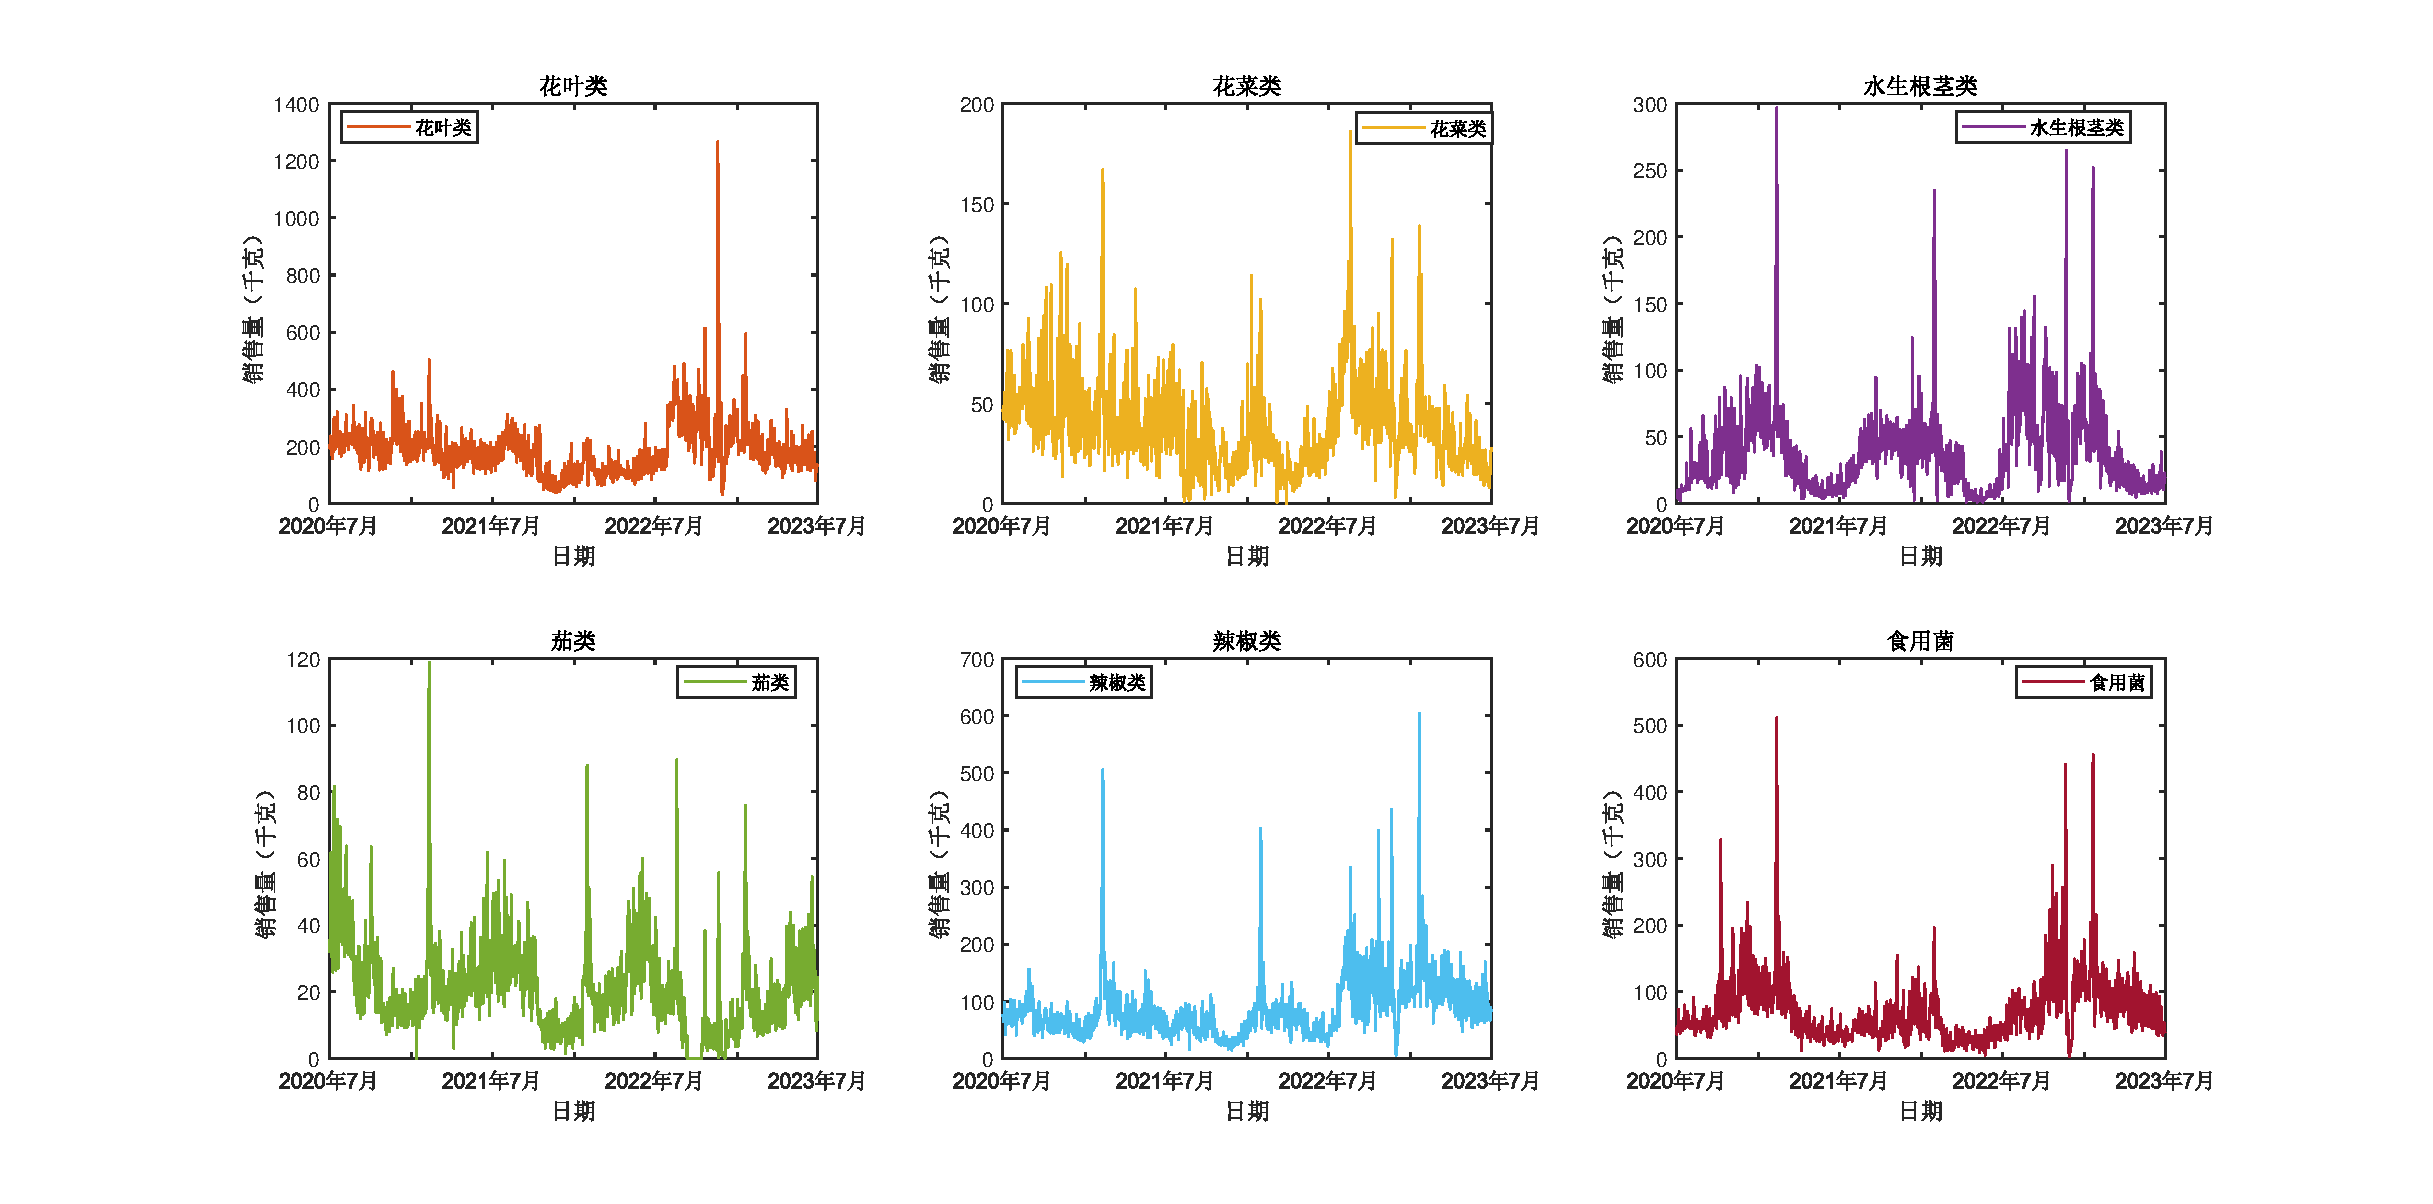
\includegraphics[width=\textwidth]{六类蔬菜日销售量.eps} %1.png是图片文件的相对路径
 \caption{六类蔬菜日销售量} %caption是图片的标题
 \label{六类蔬菜日销售量} %此处的label相当于一个图片的专属标志,目的是方便上下文的引用
\end{figure}\par
分析图\ref{各类蔬菜日销售量}和图\ref{六类蔬菜日销售量}中数据,得出不同品类蔬菜销售量的统计分布规律大致分为以下三种:
\begin{enumerate}
    \item 季节性\par
    即某种品类的蔬菜三年销售量数据在季节内具有相似的分布,不同季节销售量存在差异。典型蔬菜品类为水生根茎类和茄类,其销售量数据具有明显的季节性。每年4-10月,水生根茎类蔬菜的销售量相比剩余月份明显减少,茄类蔬菜的销售量相比剩余月份明显增加。
    \item 突变性\par
    即某种品类的蔬菜在周期内销售量较为稳定,但在少数日期销售量特别大。如图\ref{各类蔬菜日销售量}所示,在2021年2月10日、2022年1月30日和2023年1月20日三个日期,各品类蔬菜的销售量均出现突然上升,结合其均为除夕前一天可推测得,该情况是因为民众需要准备年夜饭而大规模采购蔬菜,所以使得蔬菜销售量发生突变。而2022年11月29日的销售量突变,结合疫情背景可推测得,该情况可能是因为某地疫情防控政策发生变化,民众大规模采购蔬菜造成的。
    \item 贝塔分布与非正态性\par
    对各个品类蔬菜三年内日销售量分布进行深入分析,在$K-S$检验后得到六种蔬菜日销售量的$P-P$图如下图\ref{p-p}所示:
    \begin{figure}[H]
     \centering
     \includegraphics[width=\textwidth]{p-p.png} %1.png是图片文件的相对路径
     \caption{六类蔬菜$P-P$图} %caption是图片的标题
     \label{p-p} %此处的label相当于一个图片的专属标志,目的是方便上下文的引用
    \end{figure}\par    
    发现各类蔬菜的日销售量均满足贝塔分布,因此在后续模型中需考虑到销售量和商超收益受季节因素的影响。同时对相关数据进行正态性检验,发现均不满足正态分布,因此后续分析各类蔬菜日销售量关系时不可采用Pearson相关系数分析。
\end{enumerate}
\textbf{Part2: 蔬菜单品销售量分析}\par
因不同品类蔬菜的单品数目差距显著,故先分别对每个品类的蔬菜绘制散点图,在各张散点图中选出出现频率最多的三种单品,以其销售量分布代表整个品类中单品销售量分布。\par
绘制的散点图见附件一,由散点图可知,花叶类选择云南生菜、云南油麦菜,上海青作为该类单品代表,花菜类选择西蓝花,青梗散花和枝江青梗散花作为该类单品代表;水生根茎类选择净藕(1)、洪湖莲藕(粉藕)和高瓜(1)作为该类单品代表;茄类选择紫茄子(2),青茄子(1)和长线茄作为该类单品代表;辣椒类选择芜湖青椒(1)、泡泡椒(精品) 和螺丝椒作为该类单品代表,以及食用菌选择西峡香菇(1)、金针菇(盒)和西峡花菇(1)作为该类单品代表。\par
与分析蔬菜品类类似,此处首先分别对每一类中所选单品代表,绘制出其日销售量折线图,如下所示:
\begin{figure}[H]
    \centering
    \begin{subfigure}{0.3\textwidth}
        \includegraphics[width=\linewidth]{花叶类单品销售量与时间关系.png}
        \caption{}
        \label{fig:sub1}
    \end{subfigure}%
    \hfill
    \begin{subfigure}{0.3\textwidth}
        \includegraphics[width=\linewidth]{花菜类单品销售量与时间关系.png}
        \caption{}
        \label{fig:sub2}
    \end{subfigure}%
    \hfill
    \begin{subfigure}{0.3\textwidth}
        \includegraphics[width=\linewidth]{水生类单品销售量与时间关系.png}
        \caption{}
        \label{fig:sub3}
    \end{subfigure}

    \vspace{1em} % 为了增加一些垂直间距

    \begin{subfigure}{0.3\textwidth}
        \includegraphics[width=\linewidth]{茄类单品销售量与时间关系.png}
        \caption{}
        \label{fig:sub4}
    \end{subfigure}%
    \hfill
    \begin{subfigure}{0.3\textwidth}
        \includegraphics[width=\linewidth]{辣椒类单品销售量与时间关系.png}
        \caption{}
        \label{fig:sub5}
    \end{subfigure}%
    \hfill
    \begin{subfigure}{0.3\textwidth}
        \includegraphics[width=\linewidth]{食用菌类单品销售量与时间关系.png}
        \caption{}
        \label{fig:sub6}
    \end{subfigure}
    \caption{不同品类蔬菜部分单品日销售量}
    \label{不同品类蔬菜部分单品日销售量}
\end{figure}
分析图\ref{不同品类蔬菜部分单品日销售量}中数据,得出不同品类中蔬菜单品的销售量统计分布规律大致分为以下两种:
\begin{enumerate}
    \item 季节性\par
    即某个品种的蔬菜三年销售量数据在季节内具有相似的分布,不同季节销售量存在差异。典型单品为金针菇(盒)和上海青。上海青在每年2-8月的销售量明显高于剩余月份,金针菇(盒)在每年4-10月的销售量明显低于剩余月份。
    \item 突变性\par
    即某种品类的蔬菜在周期内销售量较为稳定,但在少数日期销售量特别大。典型单品为洪湖莲藕(粉藕),其日销售量较为稳定,但每年1-2月份即过年附近,其日销售量会发生突变,年后销售量回归正常范围之内。
    \item 非正态性\par
    经过正态性检验,发现各个蔬菜单品均不满足正态分布,因此分析各个单品销售量的关系时不可采用Pearson相关系数进行分析。
\end{enumerate}
\subsubsection{各类蔬菜及单品销售量相互关系}
\textbf{Part1: 各类蔬菜相互关系分析}\par
由题可知,蔬菜类商品不同品类之间可能存在一定的关联关系,同时鉴于销售量数据具有时序性质,因此本文采用协方差分析和向量自回归模型来结合分析不同蔬菜品类销售量的相互关系。\par
\begin{equation}
    Cov(X,Y)=E[(X-E[X])(Y-E[Y])]
    \label{协方差}
\end{equation}


\begin{itemize}
    \item 根据公式\ref{协方差},计算得出六种品类蔬菜销售量的协方差矩阵,如表\ref{品类协方差矩阵}所示:
\begin{table}[H]
    \centering
    \caption{各品类蔬菜协方差矩阵}
    \label{品类协方差矩阵}
    \begin{tabular}{ccccccc}
    \toprule
        ~ & 花叶类销量 & 花菜类销量 & 水生根茎销量 & 茄类销量 & 辣椒类销量 & 食用菌销量 \\ 
        \midrule
        花叶类销量 & 7270.698 & 1212.006 & 1477.552 & 362.792 & 2974.949 & 2627.312 \\ 
        花菜类销量 & 1212.006 & 519.306 & 385.115 & 104.810 & 662.936 & 578.476 \\ 
        水生根销量 & 1477.552 & 385.115 & 972.215 & 43.242 & 1017.087 & 1021.657 \\ 
        茄类总销量 & 362.792 & 104.810 & 43.242 & 173.792 & 223.701 & 89.313 \\ 
        辣椒类销量 & 2974.949 & 662.936 & 1017.087 & 223.701 & 2857.611 & 1791.329 \\ 
        食用菌销量 & 2627.312 & 578.476 & 1021.657 & 89.313 & 1791.329 & 2387.539 \\ 
        \bottomrule
    \end{tabular}
\end{table}\par
为进一步直观分析不同品类蔬菜销量之间的关系,故进一步计算其彼此相关系数。由于前文已对数据进行过正态性检验,发现其均不满足正态分布,故不适用Pearson相关系数。同时不同数据之间的相互关系无法确定是否是线性的,因而本文最终选择计算Spearman相关系数。\par
    根据上述分析,根据相关系数计算的相关公式,计算得出不同品类蔬菜之间的相关系数,并绘制对应相关系数热力图如下:
    \begin{figure}[H]
         \centering
         \includegraphics[width=\textwidth]{类间Spearman.png} 
         \caption{六种蔬菜Spearman相关系数图} %caption是图片的标题
         \label{六种蔬菜Spearman相关系数热力图} %此处的label相当于一个图片的专属标志,目的是方便上下文的引用
    \end{figure}\par
    分析图\ref{六种蔬菜Spearman相关系数热力图}中数据,可初步分析得知各品类蔬菜的销售量相互关系如下:
        \begin{itemize}[label=$\star$]
            \item 花叶类蔬菜和其余蔬菜均呈现正相关关系,其中与花菜类蔬菜的正相关性最强;
            \item 茄类蔬菜与水生根茎类、食用菌两类蔬菜呈现负相关关系,与其余蔬菜的正相关性较弱;
            \item 辣椒类蔬菜与其余蔬菜均呈现正相关关系,其中与茄类蔬菜的正相关性最弱。
        \end{itemize}
    \item 为进一步探究类间销售量数据的相互关系,本文采用向量自回归模型(VAR)进行定量验证。向量自回归模型是多元时间序列分析中的一个基本模型,它描述了多个时间序列之间的内部动态关系,可以捕捉多个互相关联的时间序列数据之间的关系。\par
对于本题给定的$k$个时间序列,VAR模型可表示为:
\begin{equation}
    Y_t = A_1 * Y _{t-1} + A_2 * Y _{t-2}+...+A_p*Y_{t-p}+u_t
\end{equation}\par
其中,$Y_t$为销售量在时间$t$的$k*1$向量,$A_i$为$k*k$的系数矩阵,代表第$i$个滞后,$p$为模型的滞后阶数,在本文中$p=2$,$u_t$为$k*1$的误差项向量。\par
其模型思路流程图如下所示:
\begin{figure}[H]
 \centering
 \includegraphics[width=\textwidth]{VAR模型流程图.png} 
 \caption{VAR模型流程示意图} %caption是图片的标题
 \label{VAR模型流程示意图} %此处的label相当于一个图片的专属标志,目的是方便上下文的引用
\end{figure}\par

\textbf{Step1: 时间序列变量平稳性检验}\par
在采用VAR模型分析各类蔬菜相互关系之前,首先需要对各个蔬菜的销售量进行平稳性检测,若各序列均为平稳序列方可建立VAR模型,否则得到的向量自回归模型是伪回归。对时间序列变量进行平稳性检验我们通常采用ADF检验法,计算对应T检验结果,AIC值、P值等等。\par
一般来说,若 $P<0.05$,则说明序列是平稳序列; 若 $P>0.05$,则说明序列是非平稳序列。题中所给各类蔬菜销售量的ADF结果如下表所示:
\begin{table}[H]
    \centering
     \caption{向量自回归模型ADF检验}
    \begin{tabular}{cccccc}
    \toprule
        变量 & $t$ & $P$ & 临界值1\% &临界值5\%  & 临界值10\% \\ 
        \midrule
        花叶类总销量(千克) & -2.904 & 0.045** & -3.437 & -2.864 & -2.568 \\ 
        花菜类总销量(千克) & -3.018 & 0.033** & -3.437 & -2.864 & -2.568 \\ 
        水生根茎类总销量(千克) & -2.904 & 0.045** & -3.437 & -2.864 & -2.568 \\ 
        茄类总销量(千克) & -3.835 & 0.003*** & -3.437 & -2.864 & -2.568 \\ 
        辣椒类总销量(千克) & -3.607 & 0.006*** & -3.437 & -2.864 & -2.568 \\ 
        食用菌总销量(千克) & -3.415 & 0.010** & -3.437 & -2.864 & -2.568 \\ 
        \bottomrule
    \end{tabular}
    \label{ADF检验}
\end{table}
\vspace{-0.5cm}
 注:***、**、*分别代表1\%、5\%、10\%的显著性水平

由表\ref{ADF检验}可知,六类蔬菜销售量对应$P$值均小于0.05,即所有销售量序列均为平稳的时间序列,因而可以建立VAR模型。\par
\vspace{0.5cm}
\textbf{Step2: 确定模型滞后阶数}\par
在使用VAR模型时,为更好地分析各时间序列变量之间的动态关系,通常我们需要先确定模型的最佳滞后阶数,以便更精确地对模型参数进行相关估计,因此我们需根据相关判据来确定所选择的滞后阶数。\par
通常,对于VAR模型,常用的用于选择较优滞后阶数的信息准则有对数似然函数值($logL$),最终预测误差(FPE)、赤池信息准则(AIC),贝叶斯信息准则($SC$)等\textbf{准则来源的论文引用}。其中SC越小,通常意味着模型在考虑复杂性后仍具有良好的拟合性,$logL$越大,通常意味着给定模型较为适合观察到的数据。\par
鉴于题中所给附件的数据具有时序特征,同时样本量较大,因而可以同时采用$logL$和$SC$来作为判据,可以在一定程度上避免模型的过度拟合,选择出较为适宜的滞后阶数。相关滞后阶数所对应的$logL$和$SC$值如下表所示:
\begin{table}[H]
    \centering
    \caption{不同滞后阶数的比较}
    \begin{tabular}{p{2.0cm}<{\centering}p{4.0cm}<{\centering}p{2.0cm}<{\centering}}
    \toprule
        滞后阶数 & $logL$ & $SC$ \\ 
        \midrule
        0 & -30034.369 & 40.112 \\ 
        1 & -28014.21 & 36.56 \\ 
        2 & -27749.724 & 36.346* \\ 
        3 & -27610.839 & 36.371 \\ 
        4 & -27521.183 & 36.489 \\ 
        5 & -27420.258 & 36.587 \\ 
        6 & -27255.456 & 36.562 \\ 
        7 & -27152.925 & 36.656 \\ 
        8 & -27095.954 & 36.838 \\ 
        9 & -27037.521 & 37.017 \\ 
        10 & -26989.356 & 37.217 \\ 
        11 & -26934.701 & 37.404 \\ 
        \bottomrule
    \end{tabular}
    \label{不同滞后阶数的比较}
\end{table}
由表\ref{不同滞后阶数的比较}可知,在滞后阶数为2时,$SC$取得最小值,同时所对应的$logL$值相对较大,因此模型采用的滞后阶数为2阶。\par
\vspace{0.5cm}
\textbf{Step3: 模型参数估计计算}\par
由前文知,本模型采用2阶滞后系数,因而根据VAR模型的相关知识,知我们可计算出一共72个系数,其中系数的大小和正负性意味着不同销售量之间,以及该销售量与其滞后值之间的相关性。系数越大意味着滞后变量对当前变量的影响越大,系数为正意味着两个时间序列变量之间呈现正相关关系,系数为负意味着两个时间序列变量之间呈现负相关关系。\par
为了估计系数矩阵$A_1$和$A_2$,我们采取如下步骤:
\begin{enumerate}
    \item 对于每个时间点$t$,将$Y_{t-1}$和$Y_{t-2}$并列堆叠,使得矩阵$X$的每一行具有$2k$个元素;
    \item 采用最小二乘法,根据下列公式\ref{二乘法}得到估计矩阵$\hat{\mathbf{B}}$:
        \begin{equation}
            \label{二乘法}
            \hat{\mathbf{B}}=\left(\mathbf{X}^{\prime} \mathbf{X}\right)^{-1} \mathbf{X}^{\prime} \mathbf{Y}
        \end{equation}\par
    其中$\hat{\mathbf{B}}$是一个$2k*k$的矩阵,包含了$A_1$和$A_2$的估计值,$\mathbf{X}^{\prime}$代表矩阵$X$的转置。
    \item 从$\hat{\mathbf{B}}$中提取前$k$列得到$\hat{\mathbf{A}}_1$,提取后$k$列得到$\hat{\mathbf{A}}_2$,
\end{enumerate}\par
根据相关公式,计算得该模型的参数估计表如下所示:\par
\begin{table}[H]
    \centering
    \caption{参数估计表}
    \begin{tabular}{ccccccc} 
    \toprule
        参数  & $X_1$& $X_2$ & $X_3$ & $X_4$ & $X_5$ & $X_6$\\ 
        \midrule
        $X_1^{-1}$ & 0.217 & -0.01 & -0.096 & -0.024 & -0.126 & -0.112 \\
        $X_1^{-2}$ & 0.506 & 0.043 & 0.115 & 0.028 & 0.124 & 0.11 \\
        $X_2^{-1}$ & 0.48 & 0.59 & 0.136 & 0.064 & 0.207 & 0.163 \\ 
        $X_2^{-2}$ & -0.181 & 0.084 & -0.125 & -0.056 & -0.106 & -0.113 \\ 
        $X_3^{-1}$ & -0.002 & 0.031 & 0.466 & -0.016 & -0.105 & 0.025 \\ 
        $X_3^{-2}$ & -0.174 & -0.042 & 0.259 & -0.019 & -0.002 & -0.069 \\ 
        $X_4^{-1}$ & 0.211 & 0.004 & -0.211 & 0.561 & -0.105 & -0.257 \\ 
        $X_4^{-2}$ & -0.849 & -0.141 & -0.144 & 0.158 & -0.453 & -0.27 \\
        $X_5^{-1}$ & 0.212 & -0.015 & 0.102 & 0.022 & 0.645 & 0.073 \\ 
        $X_5^{-2}$ & -0.124 & -0.008 & -0.115 & -0.028 & 0.158 & -0.059 \\ 
        $X_6^{-1}$ & 0.12 & 0.045 & 0.113 & 0.005 & 0.183 & 0.61 \\ 
        $X_6^{-2}$ & -0.201 & -0.055 & -0.11 & -0.024 & -0.222 & 0.115 \\ 
        \bottomrule
    \end{tabular}
\end{table}
其中$X_i$代表花叶类、花菜类、水生根茎类、茄类、辣椒类和食用菌六类蔬菜中第i类蔬菜,$X_i^j$代表上述六类蔬菜中第i类蔬菜的第j阶滞后值。分析表中数据,发现其与通过Spearman相关系数热力图分析的结果一致,证明了相关分析的合理性。\par
\vspace{0.5cm}
\textbf{Step4: 模型稳定性检验}\par
为进一步确保上述不同品类蔬菜的关系分析准确,因此需要对该VAR模型进行稳定性检验。通常采取的方法是AR根检验法,即求解其对应特征方程的所有根,若点均落在单位圆内,则可由此判断该VAR系统是稳定的,即相关推论合理,反之相关推论则不合理。\par
根据其相关计算公式,计算其对应特征方程的所有根,并绘制AR根检验图,如下所示:
\begin{figure}[H]
 \centering
 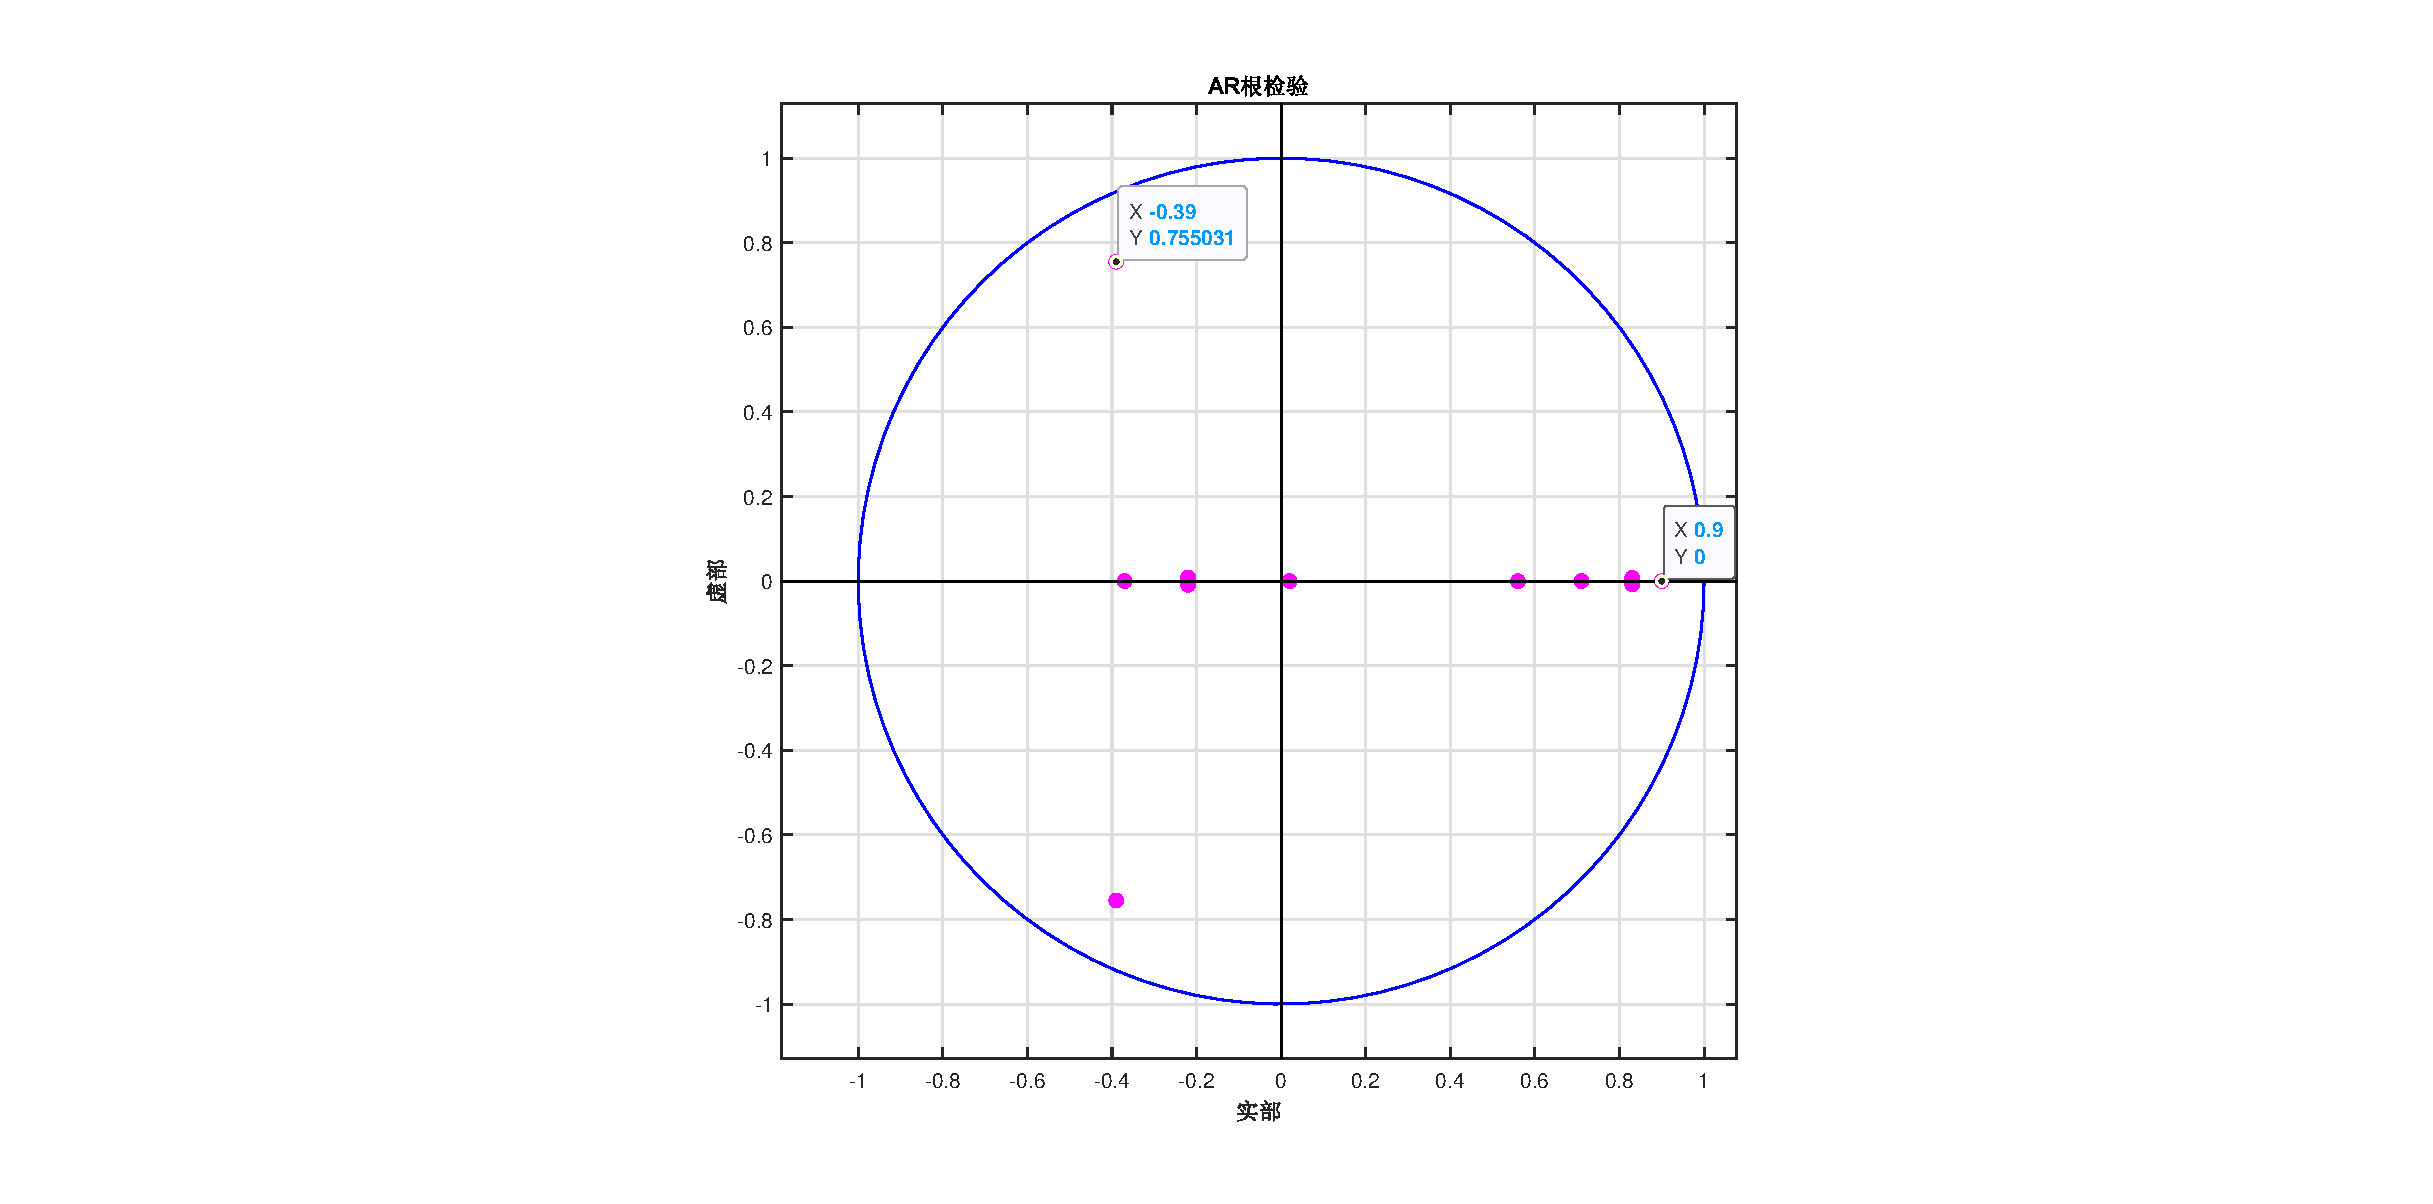
\includegraphics[width=0.8\textwidth]{AR根检验图.eps} 
 \caption{AR根检验图} %caption是图片的标题
 \label{AR根检验图} %此处的label相当于一个图片的专属标志,目的是方便上下文的引用
\end{figure}\par
由图\ref{AR根检验图}知,所有的点均落在单位圆内,即本文所建立的VAR模型是合理的,即对不同蔬菜销售量的相互关系分析有着合理性。\par
\end{itemize}
\vspace{0.5cm}
\textbf{Part2: 各种蔬菜单品相互关系分析}\par
与前文分析类似,由于单品销售量的特征和其所属蔬菜类基本一致,因此各单品的相互关系分析也采取各蔬菜类相关性分析的思路,即计算类内各单品彼此构成的协方差矩阵,并进一步计算其Spearman相关系数,并绘制对应热力图。由于不同蔬菜品类中单品数目各异,故本文中仅展示花菜类单品和茄类单品的相关系数热力图,如下所示:
\begin{figure}[H]
    \centering
    \begin{subfigure}{0.45\textwidth}
        \includegraphics[width=\linewidth]{spearman花菜类.png}
    \end{subfigure}%
    \hfill
    \begin{subfigure}{0.45\textwidth}
        \includegraphics[width=\linewidth]{spearman茄类.png}
    \end{subfigure}
    \caption{花菜类和茄类单品相关系数热力图}
    \label{花菜类和茄类单品相关系数热力图}
\end{figure}
分析图\ref{花菜类和茄类单品相关系数热力图}中数据,可初步分析得知两类蔬菜中单品销售量相互关系如下:
        \begin{itemize}[label=$\star$]
            \item 两类蔬菜中各单品的相关性不强,且若单品对应品种接近,则彼此基本呈现负相关性。
            \item 花菜类蔬菜中各单品彼此正相关性较差,两两之间大多呈现负相关,其中青梗散花和枝江青梗散花之间的负相关性最强;
            \item 茄类蔬菜中各单品彼此相关性普遍偏弱,两两之间正相关性和负相关性占比接近;部分单品如青茄子(2)和紫茄子(1)之间呈现较强的正相关性。
        \end{itemize}
        
        通过上述分析,可以得出相同蔬菜品类中的不同单品存在的相互关系:彼此基本呈现负相关性,即不同蔬菜单品之间存在相互替代的关系。
\subsection{问题二模型的建立与求解}
\subsubsection{蔬菜品类销售总量与成本加成定价关系}
由于需要分析各蔬菜品类的销售总量与成本加成定价的关系,同时考虑到不同蔬菜品类中各单品占整个品类的成本加成定价的比例不同,因而我们需要分析各单品成本加成定价占总体的权重,以便计算各类蔬菜的总体成本加成定价。\par
\textbf{Part1:各单品利润比例计算}\par
首先我们根据模型准备处给出的利润计算公式,分别计算出各品种蔬菜每日的利润值,并基于单品利润计算其在品类整体利润中所占比例。\par
\vspace{0.5cm}
\textbf{Part2:单品占品类利润的权重分析}\par
基于计算得到的利润比例,对于每个品类内的各个单品,对其成本加成定价进行加权处理并做累加,最终结果即该品类的成本累和形成定价。\par
\vspace{0.5cm}
\textbf{Part3:各品类销售总量与成本加成定价关系分析}\par
在计算得出各品类的成本加成定价后,采用相关系数对其相互关系进行分析。根据问题假设,对商品补货量的分析可等价为对商品销售量的分析。在进行相关系数分析时,需要进行相关检验,以便确定选择相关系数种类。就本小问而言,先对六类蔬菜成本加成定价进行正态性检验,包括S-W检验和K-S检验,得到结果如下表所示:
\begin{table}[H]
    \centering
     \caption{蔬菜成本加成定价正态性检验}
    \begin{tabular}{cccccc}
    \toprule
        变量 & S-W检验  & K-S检验 \\ 
        \midrule
        花叶类加成定价 & 0.014(0.000***) & 0.491(0.000***) \\
        花菜类加成定价 & 0.756(0.000***) & 0.096(0.000***) \\
        水生根茎类加成定价 & 0.138(0.000***) & 0.362(0.000***) \\
        茄类加成定价 & 0.959(0.000***) & 0.073(0.000***) \\
        辣椒类加成定价 & 0.711(0.000***) & 0.157(0.000***) \\
        食用菌加成定价 & 0.982(0.000***) & 0.027(0.386) \\
        \bottomrule
    \end{tabular}
    \label{加成定价整体性检验}
\end{table}
\vspace{-0.5cm}
 注:***、**、*分别代表1\%、5\%、10\%的显著性水平\par
 由表\ref{加成定价整体性检验}可知,各类蔬菜的成本加成定价均不满足正态分布,故应当选择Spearman相关系数进行分析,根据相关系数的公式,计算得到并绘制热力图如下:
 \begin{figure}[H]
 \centering
 \includegraphics[width=\textwidth]{成本加成定价热力图.png} 
 \caption{成本加成定价热力图} %caption是图片的标题
 \label{成本加成定价热力图} %此处的label相当于一个图片的专属标志,目的是方便上下文的引用
\end{figure}\par
由图\ref{成本加成定价热力图},经分析可初步得知以下有关成本加成定价和销售量即补货量之间的关系结论:
\begin{itemize}
    \item 对同一类蔬菜而言,其总销量和成本加成定价之间均呈现负相关关系,即总销量越高,成本加成定价越低,反之亦然;
    \item 对于同一种类数据而言,不同种蔬菜的总销量之间通常呈现正相关关系,成本加成定价之间相关系偏弱,负相关占有一定比例。
\end{itemize}
\subsubsection{基于季节性ARIMA模型的蔬菜品类补货量预测}
由于前文分析得知各品类蔬菜的销售量满足贝塔分布,即需要考虑季节性因素对销售量的影响,因此本问采用季节性ARIMA模型(SARIMA)进行蔬菜补货量的预测\cite{nosek2002math},其建模流程图如下所示:
\begin{figure}[H]
 \centering
 \includegraphics[width=\textwidth]{SARIMA流程图.png} 
 \caption{SARIMA流程图} %caption是图片的标题
 \label{SARIMA流程图} %此处的label相当于一个图片的专属标志,目的是方便上下文的引用
\end{figure}\par
\begin{itemize}
    \item \textbf{平稳性检验与处理:}\par
    SARIMA模型要求序列本身满足平稳性\cite{22},故在进行预测之前需采用ADF检验的方式判断数据是否平稳。\par
    若数据不平稳则可采取多次差分的方式使不平稳的数据平稳化,并可根据AIC值等评价指标来决定最终采用几阶差分处理,AIC值越小模型拟合效果越好。就本题而言,以花叶类补货量为例,其ADF检验表如下所示:
    \begin{table}[H]
    \centering
    \caption{花叶类补货量ADF检验表}
    \begin{tabular}{cccccccc}
    \toprule
    变量 & 差分阶数 & t & P & AIC & 临界值1\% & 临界值5\% & 临界值10\% \\ 
        \midrule
        花叶类总销量(千克) & 0 & -2.825 & 0.055* & 11693.589 & -3.437 & -2.864 & -2.568 \\ 
        ~ & 1 & -11.771 & 0.000*** & 11688.618 & -3.437 & -2.864 & -2.568 \\ 
        ~ & 2 & -15.09 & 0.000*** & 11773.384 & -3.437 & -2.864 & -2.568 \\ 
        \bottomrule
    \end{tabular}
    \label{ADF检验表}
\end{table}
    由表\ref{ADF检验表}知,不进行差分处理时其P值为0.055>0.05,即该序列并不平稳,但在一阶差分后该序列便已经平稳。同时考虑到AIC值,故对该补货量数据采用一阶差分处理。\par
    处理完成后,对一阶差分后的平稳序列进行白噪声检验,分析得六类蔬菜的相关序列成功通过检验,故可以用于预测数据。
    \item \textbf{模型拟合估计:}\par
    本文使用SPSS PRO对模型进行拟合定阶,最终确定采用SARIMA(5,1,1)模型进行分析,以花叶类补货量为例,其模型参数表如下所示:
    \begin{table}[!ht]
    \centering
    \caption{拟合优度表}
    \begin{tabular}{p{2.0cm}<{\centering}p{3.0cm}<{\centering}p{3.0cm}<{\centering}}
    \toprule
        项 & 符号 & 值 \\ 
        \midrule
        \multirow{2}*{信息准则} & AIC & 12080.948 \\ 
        ~ & BIC & 12120.856 \\ 
        拟合优度 & R² & 0.664 \\ 
        \bottomrule
    \end{tabular}
\end{table}
    由该表可知,该模型的拟合优度很接近1,故模型很好满足相关要求,可以用于预测相关数据。
    \item \textbf{预测评价:}\par
    根据上述分析,采用该模型对六类蔬菜在2023年7月1日至7月7日的补货量进行预测得到结果如表\ref{各品类蔬菜未来一周建议日补货量}所示:
    \begin{table}[H]
    \centering
    \caption{各品类蔬菜未来一周建议日补货量}
    \begin{tabular}{cccccccc}
    \toprule
        日期 & $X_1$(kg) & $X_2$(kg) & $X_3$(kg) & $X_4$(kg) & $X_5$(kg) & $X_6$(kg) & ~ \\
        \midrule
        2023-07-01 & 125.4~ & 24.1~ & 22.1~ & 22.1~ & 84.2  &   43.5 ~  \\ 
        2023-07-02 & 116.1~ & 16.2~ & 14.3~ & 19.2~ & 71.3~ &   35.3~ \\ 
        2023-07-03 & 114.8~ & 15.5~ & 12.5~ & 18.5~ & 63.9~ &   30.9~ \\ 
        2023-07-04 & 106.2~ & 17.7~ & 12.8~ & 17.2~ & 60.2~ &   30.3~ \\ 
        2023-07-05 & 136.2~ & 20.3~ & 17.9~ & 19.3~ & 68.8~ &   35.6~ \\ 
        2023-07-06 & 158.1~ & 25.5~ & 23.2~ & 23.4~ & 85.9~ &   45.1~ \\ 
        2023-07-07 & 166.3~ & 26.8~ & 26.3~ & 25.8~ & 88.2~ &   46.9~ \\ 
        \bottomrule
    \end{tabular}
    \label{各品类蔬菜未来一周建议日补货量}
\end{table}
\end{itemize}

\subsubsection{补货总量与定价策略}
从商超角度出发,需要在保证收益最大情况下尽可能提升自身利润率,增加每日蔬菜销售量,减少运输过程中蔬菜损耗率和消费者退货造成的收益损失\cite{33}。题中要求使得商超一周收益最大,由于不考虑库存影响,本文将其进行离散化处理,以单日的商超总利润为优化目标,以蔬菜销售量、利润率范围和定价与销售量关系作为约束条件,以成本加成利润率作为决策变量,以蔬菜运输损耗和退货收益损失为环境参量。模型总体示意图如图\ref{蔬菜品类定价模型示意图}所示:
\begin{figure}[H]
 \centering
 \includegraphics[width=\textwidth]{品类定价策略优化.png}
 \caption{蔬菜品类定价模型示意图} %caption是图片的标题
 \label{蔬菜品类定价模型示意图} %此处的label相当于一个图片的专属标志,目的是方便上下文的引用
\end{figure}\par
\begin{itemize}
    \item \textbf{确定决策变量}\par
    本问需规划利润最大的情况下各品类日补货总量和定价策略,故以成本加成定价的利润率$r_i$作为决策变量。
    \item \textbf{确定优化目标}\par
    本问中要求商超利润最大化,故优化目标为商超总利润$W$,记$C_i$为第$i$品类的成本,$M_i$为第$i$品类的销售总量。优化目标为:\\
    \begin{equation}
        maxW=\displaystyle\sum_{i=1}^{6} r_iC_iM_i
    \end{equation}
    \item \textbf{确定约束条件}\par
    (1)由于蔬菜销售量的变化在一定范围内波动,因此各个品类的销售量不超过一个月内该品类的最大销售总量。即
    \begin{equation}
        M_i\leq M_{imax}
    \end{equation}
    (2)商超以盈利为目标,故利润率$r_i$,销售量$M_i$大于零, 
    \begin{equation}
        0< r_i < r_i|_{M_i=0}
    \end{equation}
    (3) 销售量与定价之间存在定量关系,根据6.2.2的结论,采用三次样条插值对成本加成定价和总销售量进行拟合,得到二者的关系为
    \begin{equation}
        P_i=\begin{cases}
            \alpha_1 M_i^3+\beta_1 M_i^2+\gamma_1 M_i+\lambda_1,& M_i\in[R_1,R_2]\\
            \alpha_2 M_i^3+\beta_2 M_i^2+\gamma_2 M_i+\lambda_2,& M_i\in[R_2,R_3]\\
            \alpha_3 M_i^3+\beta_3 M_i^2+\gamma_3 M_i+\lambda_3,& M_i\in[R_3,R_4]\\
        \end{cases}      
    \end{equation}
        $$\text{又有}P_i=(1+r_i)C_i$$
        $$\text{则}r_i=\frac{P_i}{C_i}-1$$
    (4)考虑到有退货影响,本文认为退货后的商品不再进行出售,视作损失,将品类$i$单日发生退货的量记为$\hat{X_i}$,通过K-S检验发现退货服从泊松分布,因此将$\hat{X_i}$视为随机变量影响。那么品类$i$的泊松分布型退货函数为$f(\hat{X_i})$。

    综上所述,补货总量与定价策略规划模型为:
    $$  maxW=\displaystyle\sum_{i=1}^{6} r_iC_iM_i $$
    \begin{equation}      
        s.t.\begin{cases}
             M_i\leq M_{imax},\\
             0< r_i < r_i|_{M_i=0},\\
             r_i=\frac{P_i}{C_i}-1,i=1,2,...,6\\
        \end{cases}
    \end{equation} 
\end{itemize}
\subsubsection{基于动态权重的离散化贪心和动态规划算法的模型求解}
\begin{itemize}
    \item \textbf{算法分析:}\par
    \hspace{2em}就动态权重而言,因题目需计算未来一周的最大收益,而不同日期售卖蔬菜单品不同,若整周采取固定权重,可能会导致最初收益较大但总体收益较低的情况。因而对于每天的收益而言,需要动态调整成本加成定价中各品类蔬菜的权重。\par
    \hspace{2em}就动态规划而言,全过程均使用动态规划算法以便求得全局最优解,具体为:
\begin{equation}
    DP[i]=\max \left(DP[i], T(x, w_{it})+T\left(i-x, w_{it}^{\prime}\right)\right)
\end{equation}
\hspace{2em}其中,$DP[i]$为当前为周内第i天时此时的最优策略,$T$为贪心规划过程,$x$和$i-x$表示在此次贪心过程中经过了多少天,二者保证两次贪心规划的天数不重复,$w_{it}$代表周内第i种蔬菜第t天对该品类成本加成定价的权重,$w_{it}^{\prime}$代表前一部分贪心规划后,更新的相应权重。\par
\hspace{2em}就离散化规划而言,因每天各品类蔬菜的补货量各不相同,因而可以使用离散化规划的方法。首先根据各品类蔬菜每天的期望补货量产生离散化数据, 以其补货量,销售量,损耗率和售价等等作为一个数据结构单位。对所有品类的蔬菜都进行此离散化处理, 以便于后续的排序与选择。
\item \textbf{模型求解与分析:}\par
\hspace{2em}根据上述算法,使用Python 3.9 求解得出相关结果,计算得未来一周最大收益为12如下表所示:
\begin{table}[H]
    \centering
    \caption{花菜类商品补货量}
\begin{tabular}{ccc}
\hline 日期 &  日补货总量 (千克) & 定价策略 \\
\hline 2023-07-01 & 53.4 & 49.21\% \\
2023-07-02 & 20.3 & 26.23\% \\
2023-07-03 & 41.3 & 48.21\% \\
2023-07-04 & 39.4 & 87.36\% \\
2023-07-05 & 50.9 & 42.26\% \\
2023-07-06 & 31.6 & 38.83\% \\
2023-07-07 & 29.2 & 53.22\% \\
\hline
\end{tabular}
\end{table}
剩余五种品类的结果放置在附录
\end{itemize}
\subsection{问题三模型的建立与求解}
\subsubsection{数据筛选与处理}
根据题意知,该问题是基于2023年6月24日至6月30日商超的可售品种进行分析,且单品总数和陈列量存在限制,因此对于附件中的蔬菜单品可依据如下依据进行预筛选筛选:
\begin{itemize}
    \item 若某蔬菜单品在该段时间内补货量均为0,则将其视作这段时间内不可售,因而无需考虑;
    \item 若某蔬菜单品在该段时间内利润占总利润比例低于1\%,即出售该单品的性价比过低,因而无需考虑。
\end{itemize}
\subsubsection{基于GM(2,1)的单品销售相关数据预测}
由题可知,需根据2023年6月24日至6月30日商超的可售品种,以给出7月1日商超的单品补货与定价策略。考虑到仅7日的数据样本量过小,难以使用传统ARIMA模型或者是机器学习类模型,且数据在短时间内不具有季节性,因此本问采用GM(2,1)模型进行预测,预测流程图如下所示:
\begin{figure}[H]
 \centering
 \includegraphics[width=\textwidth]{GM(2,1)流程图.png} 
 \caption{GM(2,1)预测流程图} %caption是图片的标题
 \label{GM(2,1)流程图} %此处的label相当于一个图片的专属标志,目的是方便上下文的引用
\end{figure}\par
由图\ref{GM(2,1)流程图}可知,可分为以下三个部分:
\begin{enumerate}
    \item \textbf{计算均值序列:}\par
对于每一种蔬菜$x_i$,其对应数据序列我们记作$x_i^{(0)}=\left(x_i^{(0)}(1), x_i^{(0)}(2), \cdots, x_i^{(0)}(n)\right)$,接着计算其 1-AGO 序列和1-IAGO 序列,然后根据公式\ref{均值生成序列}
\begin{equation}
    \label{均值生成序列}
    z^{(1)}=\left(z_i^{(1)}(2), z_i^{(1)}(3), \cdots, z_i^{(1)}(n)\right)
\end{equation}
计算得到其紧邻均值生成序列。
\item \textbf{最小二乘法拟合参数:}\par
首先根据其均值生成序列求得白化矩阵,然后根据最小二乘法计算得到其中一个参数,随后根据公式\ref{参数a}
\begin{equation}
    \label{参数a}
    \frac{d^2x_i^{(1)}(t)}{dt^2}+a_1\frac{d^2x_i^{(1)}(t)}{dt}=b
\end{equation}
求解得到另一个参数,从而得到GM(2,1)模型的时间响应式。
\item \textbf{反累加最终预测:}\par
由已有6月24日-6月30日的相关数据,带入表达式得初次预测序列,再对该序列进行一次反累加操作,得到新序列,该序列即下一个元素预测值。\par
通过上述方法,最终得到各产品的部分相关信息如下表示:
\begin{table}[H]
    \centering
    \caption{部分产品预测信息}
    \begin{tabular}{ccccccc}
    \toprule
         & 单品编码 & 销量(千克) & 批发价格(元/干克) & 售价(元/干克) &   品名 & 补货量 \\
    \midrule
    & 102900005116257 & 18.9 & 4.22 & 6.09  & 紫茄子(2) & 19.87 \\
     & 102900005116899 & 10.4 & 6.81 & 11.13  & 净稞(1) & 10.79 \\
     & 102900005116714 & 25.3 & 9.63 & 14.42  & 西兰花 & 28.23 \\
     & 102900011030059 & 40.2 & 3.08 & 4.37  & 云南生菜(份) & 44.41 \\
    & 102900005118831 & 16.1 & 4.39 & 6.59  &  娃娃菜 & 16.80 \\
    & 102900011031100 & 27.6 & 2.81 & 6.43  &  小米椒(份) & 30.02 \\
    & 102900051000944 & 4.8 & 17.88 & 22.20  &  洪湖藕带 & 5.92 \\
    \bottomrule
    \end{tabular}
\end{table}
\end{enumerate}



\subsubsection{单品补货方案与定价策略}
\begin{itemize}
    \item \textbf{确定决策变量}\par
决策变量应为是否对某种单品进行补货,故引入$0-1$整数变量表示如下:
\begin{equation}
    s_i=\begin{cases}
        1,&\text{选择第}i\text{种单品}\\
        0,&\text{否则}
    \end{cases}
\end{equation}
\item \textbf{确定优化目标}\par
本问中需要选择$27-33$种蔬菜单品,使得商超利润达到最大,故优化目标为:
\begin{equation}
    maxW=\displaystyle\sum_{i=1}^{49} s_ir_iC_iM_i
\end{equation}
\item \textbf{确定约束条件}\par
(1)单品订购量需满足最小陈列量2.5kg的要求,则
\begin{equation}
    M_i \geq 2.5
\end{equation}
(2)选取的单品数量要在27-33种之间,因此
\begin{equation}
   27\leq \displaystyle\sum_{i=1}^{49} s_i \leq 33
\end{equation}
(3)分析所给数据得,7.1可能发生退货,因此也需要考虑随机变量影响,记$\hat{Y_i}$为单品$i$产生退货的数量,则对单品$i$的泊松分布型退货函数为 $f(\hat{Y_i})$

(4)题中要求各品类蔬菜都有,且要满足对各品类的需求,因此有
\begin{equation}
    S_i \geq 1,\displaystyle\sum_{j=1}^{s_i}M_j\geq M_{jmin}
\end{equation}
综上可得,单品补货量和定价策略规划模型为:
$$maxW=\displaystyle\sum_{i=1}^{49} s_ir_iC_iM_i$$
 \begin{equation}      
        s.t.\begin{cases}
             M_i \geq 2.5,\\
             27\leq \displaystyle\sum_{i=1}^{49} s_i \leq 33,\\
             f(\hat{Y_i})\\
             S_i \geq 1,\\
             \displaystyle\sum_{j=1}^{s_i}M_j\geq M_{jmin}\\
             \hat{Y_i}\geq M_i\\
             M_j\geq M_{jmin}
        \end{cases}
    \end{equation}
\end{itemize}
\subsubsection{基于分支限界的0-1背包动态规划算法的模型求解}
\begin{itemize}
    \item \textbf{算法分析:}\par
\hspace{2em}就0-1背包问题而言,在满足其余约束条件的情况下,我们更倾向于选择单位利润更高的单品。同时因可售单品总数具有相关限制,因而我们可以写出对应状态转移方程如下:
\begin{equation}
DP(j)=\max (DP(j), DP(j-S_p(i))+V(i))
\end{equation}
其中$S_p(i)$ 为第$\mathrm{i}$种单品占用销售空间, $V(i)$ 为第 $\mathrm{i}$ 种单品的利润。\par
算法思路如下图所示:
\begin{figure}[H]
 \centering
 \includegraphics[width=\textwidth]{分支限界流程图.png} 
 \caption{基于分支限界的0-1背包动态规划算法流程图} %caption是图片的标题
 \label{基于分支限界的0-1背包动态规划算法} 
\end{figure}\par
由图\ref{基于分支限界的0-1背包动态规划算法}可知,该算法的实现流程如下所示:
\begin{enumerate}
    \item Step1: 分析所预测得到的单品利润,按照从大到小顺序初始化单品利润序列;\par
    \item Step2: 选择规划的蔬菜类型, 确定初始的补货序列, 满足相关约束条件下,尽可能补货上架高利润的蔬菜单品;
    \item Step3: 根据确定的规划顺序, 应优先规划利润高的蔬菜品类,并更新对应剩余销售空间, 根据此时剩余单品空间进行分支限界,去除超过超过销售空间的可能情况,对于剩余情况继续按照0-1背包求解, 求解完毕后更新已被规划的蔬菜单品,从而防止此蔬菜单品再次被规划;\par
    \item Step4: 若当前蔬菜品类全部规划完毕,且仍有待规划蔬菜单品,则返回 Step3规划下一个蔬菜品类,若蔬菜类型未规划完毕则同样返回Step3规划下一种材料。若完全规划完毕则进入Step5;\par
    \item Step 5:输出具体数据至表格。
\end{enumerate}

    \item \textbf{模型求解与分析:}\par
    \hspace{2em}根据上述算法,使用Python 3.9 求解得出相关结果,部分结果如下表所示,剩余结果见附录:
    \begin{table}[H]
    \caption{单品销售数据}
    \centering
    \begin{tabular}{cccccc}
    \toprule
        单品编码 & 日补货总量(kg) & 定价策略\% &单品编码 & 日补货总量(kg) & 定价策略\%\\ 
        \midrule
        102900005115779 & 10.44 & 144.23\% & 102900011035740 & 1.29 & 85.37\% \\ 
        102900011033944 & 3.15 & 136.72\% & 102900011021842 & 7.37 & 79.14\% \\ 
        102900011030110 & 15.26 & 134.52\% & 102900011034231 & 13.45 & 75.94\% \\ 
        102900005115878 & 9.01 & 132.44\% &106949711300259 & 20.84 & 74.31\% \\ 
        102900005116899 & 24.97 & 128.76\% &  102900011030905 & 1.36 & 63.36\% \\ 
        102900011013274 & 2.39& 128.22\% & 102900005116714 & 18.03 & 61.12\% \\ 
        102900011023464 & 5.31 & 127.20\%  & 102900005122654 & 2.12 & 58.97\% \\ 
        102900011031100 & 19.87 & 118.75\% &  102900011016701 & 26.91 & 58.49\% \\ 
        102900011031216 & 13.56 & 118.58\% & 102900011034439 & 5.66 & 58.37\% \\ 
        102900005115625 & 3.172 & 101.84\%  &102900011034330 & 10.21 & 53.14\% \\ 
        102900011035078 & 2.762 & 101.07\%  &102900005116257 & 2.29 & 48.21\% \\ 
        102900011030059 & 13.69 & 97.27\%  &  102900005116530 & 17.72 & 47.46\% \\ 
        102900011030097 & 9.28 & 96.31\% &102900011008164 & 6.47 & 39.61\% \\ 
        102900005115861 & 18.215 & 96.02\% &   102900051000463 & 4.01 & 38.77\% \\ 
        102900051010455 & 7.795 & 92.43\%  &~   &~&~\\
        \bottomrule
    \end{tabular}
\end{table}
\end{itemize}
\subsection{问题四模型的建立与求解}
采集的其他数据目的是为了更好地制定商品的补货和定价决策,本题围绕供给侧和需求侧展开分析。供给侧方面,从商家自身考虑,为了防止新鲜度降低造成蔬菜商品滞销,商家需要尽可能快地将当天补货出售,同时需要注意仓储成本,因此本题着重考虑蔬菜商品新鲜度变化的规律以及计算仓储成本带来的影响;需求侧方面,消费者对于蔬菜商品着重考虑新鲜度和价位,消费者更愿意接收新鲜度高的蔬菜商品,因此围绕消费者心理展开。
\subsubsection{考虑新鲜度变化}
消费者在进行蔬菜选购的时候,首先会通过观察蔬菜的质量、品相以及腐烂程度等,来判断蔬菜的新鲜度。当蔬菜新鲜度较低时,会造成该类蔬菜滞销甚至被退货。通过分析题中数据,对较不新鲜的蔬菜打折,能使滞销的蔬菜尽可能多得被售出,因此在原有的定价策略上考虑蔬菜新鲜度的动态变化过程,并基于此实现动态定价策略能够进一步增加商超收益,如图\ref{基于新鲜度的动态定价过程}所示即基于新鲜度的蔬菜动态定价过程。

\begin{figure}[H]
 \centering
 \includegraphics[width=\textwidth]{新鲜度变化.png} 
 \caption{基于新鲜度的动态定价过程} %caption是图片的标题
 \label{基于新鲜度的动态定价过程} %此处的label相当于一个图片的专属标志,目的是方便上下文的引用
\end{figure}\par

建立一个蔬菜新鲜度随时间变化的模型,依据该模型对蔬菜定价进行动态调整。分析题中数据,发现该商超最早一单交易时间晚于早上9点,最晚一单交易时间早于晚上10点,即可推断该商超的营业时间为9:00-22:00,即为当天所有蔬菜产品的销售周期。同时由题可知蔬菜的进货交易时间通常为凌晨3:00-4:00,故在商品送达至商品售出前存在至少5小时的时间间隔。将该间隔考虑后,我们将蔬菜的销售周期被划分为新鲜期和新鲜度降低期,不同类别的蔬菜新鲜度衰退速度不同。规定$t_f$为分界点,假设起始时间点为0也就是凌晨4:00,$(0,t_f]$时蔬菜产品新鲜度维持高位且没有变化,在该点之后蔬菜产品的新鲜度开始降低,并设置多个新鲜度阶段,其中$(t_{i-1},t_i]$为一个销售阶段,在同一销售阶段内蔬菜价格相同。

此外,蔬菜新鲜度与其价值损耗率相关,通过数学方法可以量化新鲜度与价值损耗率的关系。设定参数$\theta \in [0,1]$表征产品的新鲜度,由于对数函数具有过$(1,0)$点、在$(0,+\infty)$上单调递增,可以构造出$\theta-\lambda(t)$的数学关系:
\begin{equation}
\lambda(t)=-ln \theta \cdot \theta^t
\end{equation}\par
其中,$\lambda(t)$表示商品价值损耗率,上式表明了蔬菜价值损耗与新鲜度的关系,因此在商品新鲜度下降后,由于商品自身价值下降,消费者的偏好程度下降,重新定价、打折出售才能与商品自身价值匹配,保持消费者的偏好程度。定义$S_i$为某一时间点的折扣,则有商品售价公式:
\begin{equation}
    P=\left\{\begin{array}{cl}
P & t \in\left(0, t_f\right] \\
S_i \cdot P & t \in\left(t_{i-1}, t_i\right]
\end{array}\right.
\end{equation}

\subsubsection{考虑消费者心理}
消费者对于某些蔬菜产品有特殊需求,同时对于某一蔬菜产品存在理想价位,此外对于产品的新鲜度格外敏感;在某些情况下,商品较低的价格能够掩盖商品新鲜度不高的缺点,激发消费者购买欲望。因此在制定蔬菜商品补货和定价决策时,需要联合考虑消费者的需求及特点。

消费者关注的是蔬菜商品的新鲜度变化以及时间偏好,考虑消费者需求的时候要注意商品新鲜度的变化。综合前文新鲜度相关描述,定义$m(t)$为消费者随时间变化的偏好函数,由于随着时间的变化,商品新鲜度降低,消费者的偏好迅速降低,可以用指数函数来刻画这一过程:
\begin{equation}
m(t)=\left\{\begin{array}{cl}
1 & t \in\left(0, t_f\right] \\
s e^{-f\left(t-t_f\right)} & t \in\left(t_{i-1}, t_i\right]
\end{array}\right.
\end{equation}

其中,$s \in (0,1)$为商超服务水平因子;$f \in (0,1)$为新鲜度变化因子,表示的是蔬菜商品的新鲜度变化程度。$(0,t_f]$间,商品新鲜度维持高位,消费者偏好程度最高为1;$(t_{i-1},t_i]$一个阶段内消费者偏好程度为离散量$s e^{-f\left(t-t_f\right)}$。消费者偏好程度的下降会造成商品销售量的下降,因此在整个销售周期内,单位时间的销售量是单调递减的,设置一个新鲜度影响因子$k_i$,表示在某一时间点因为新鲜度改变对销售量造成的影响。

\subsubsection{考虑仓储成本}
当蔬菜商品属于待售状态时,商超需要付出仓储成本。在生鲜超市中,货架数量固定且蔬菜商品不完全陈列在货架上,在商品售出一定数量之后,需要人工从仓库中取出补货。定义$h$为单位仓储成本,随着蔬菜商品进货量增加、仓储时间延长,仓储成本越高,因此在计算成本加成定价的过程中需要增加该项成本:
\begin{equation}
    P_i=(C_i+h)(1+r_i)
\end{equation}

此外还要考虑进货总量对仓储成本造成的影响,已知单品的销售量与成本加成定价存在负相关的关系,进货量的增加势必会提高仓储成本,造成售价上涨,进而引发销售量的变化,最终形成动态平衡。

\subsubsection{采集的数据对商超收益的影响}
\begin{itemize}
    \item 对于新鲜度变化\\不考虑其他因素的影响下,通过计算机模拟合理赋值,计算得的收益减少5.3\%;
    \item 对于消费者需求\\不考虑其他因素的影响下,通过计算机模拟合理赋值,计算得的收益减少7.6\%;
    \item 对于仓储成本\\不考虑其他因素的影响下,通过计算机模拟合理赋值,计算得的收益减少1.5\%;
    \item 对于新鲜度变化和消费者需求综合考虑\\新鲜度的变化会改变消费者需求,通过计算机模拟,合理调整折扣数,最终计算得的的收益增加1.8\%;
    \item 对于新鲜度变化、消费者需求和仓储成本的综合考虑\\通过计算机模拟合理赋值,计算得的收益减少0.4\%,基本与原收益持平。
\end{itemize}







\section{七、模型的评价和推广}
\subsection{模型的评价}
\subsubsection{模型的优点}
\begin{enumerate}
    \item 分析蔬菜各品类及单品销售量的分布规律及相互关系时,坚持定性与定量相结合,同时对于销售量数据进行了统计性质上的详细分析,避免错误使用某类相关系数致使相互关系分析不当;
    \item 分析各蔬菜品类的销售总量与成本加成定价的关系时,考虑到同一品类中不同单品对总体成本加成定价的贡献率不同,故采用基于利润占比加权的方式计算得到更为恰当的品类成本加成定价;
    \item 分析不同情况下商超的最佳收益时,采用复合的动态规划模型,更不容易陷入局部最优解。
\end{enumerate}
\subsubsection{模型的缺点}
\begin{enumerate}
    \item 在问题二、问题三对商超收益的分析中简单地将同一天内商品价格与时间的关系视作不连续的函数关系;
    \item 在问题二、问题三对商超收益的分析中忽略了商超彼此竞争、顾客心理选择等因素对蔬菜类商品补货和定价决策的影响。
\end{enumerate}

\subsection{模型的改进}
\begin{enumerate}
    \item 问题一中主要采取的定量分析模型为VAR模型,可以尝试其余分析模型,并对结果进行综合比较;
    \item 对商超收益的优化模型中可以尝试挖掘更多潜在的约束条件,以便更精确地分析商超收益最大的情况。
\end{enumerate}
\newpage
%------ 参考文献 ----------
\bibliographystyle{unsrt} 
\begin{center}
\bibliography{reference} 
\end{center}

%----------- 附录 ----------
\newpage
\section{附录}

\begin{table}[htbp]
    \centering
    \begin{tabular}{|p{14.0cm}|}

    \hline
    \textbf{附录1} \\ %换行 
    \hline
    .py文件是使用的python代码 \\ 
     .xls文件为本文使用的数据图表\\
     .png文件是中间过程图片
    \hline
    \end{tabular}
\end{table}
\newpage
\begin{table}[H]
    \centering
    \begin{tabular}{|p{14.0cm}|}
    \hline
    \textbf{附录2} \\ 
    \hline
\begin{lstlisting}
import pandas as pd
from tqdm import tqdm
import warnings
warnings.filterwarnings("ignore")

dataset=pd.read_csv("单品利润占比_修改缺失.csv")
shoujia=pd.read_excel("SixKindsAll.xlsx",sheet_name="Sheet1")


huaye="花叶类"
huacai="花菜类"
shuisheng="水生根茎类"
qielei="茄类"
lajiao="辣椒类"
shiyongjun="食用菌"

huaye_sunhao=12.83
huacai_sunhao=15.51
shuisheng_sunhao=13.65
qielei_sunhao=6.68
lajiao_sunhao=9.24
shiyongjun_sunhao=9.45

# print(dataset)
date = dataset.iloc[:, 0]
date.drop_duplicates(keep='first', inplace=True)
date.reset_index(drop=True, inplace=True)

result=pd.DataFrame()


for i in tqdm(range(len(date))):
    price={'日期':date[i]}
    data=dataset[dataset['日期']==date[i]]
    # print(data)

\end{lstlisting}
    \\
    \\
\hline
    \end{tabular}
\end{table}
\newpage

\begin{table}[H]
    \centering
    \begin{tabular}{|p{14.0cm}|}
    \hline
    \textbf{附录2} \\ 
    \hline
\begin{lstlisting}
huaye_data=data[data['分类名称']==huaye]
huacai_data=data[data['分类名称']==huacai]
shuisheng_data=data[data['分类名称']==shuisheng]
qielei_data=data[data['分类名称']==qielei]
lajiao_data=data[data['分类名称']==lajiao]
shiyongjun_data=data[data['分类名称']==shiyongjun]

price['花叶类加权定价']=huaye_data['售价*利润权重'].sum()
price['花菜类加权定价']=huacai_data['售价*利润权重'].sum()
price['水生根茎类加权定价']=shuisheng_data['售价*利润权重']
.sum()
price['茄类加权定价']=qielei_data['售价*利润权重'].sum()
price['辣椒类加权定价']=lajiao_data['售价*利润权重'].sum()
price['食用菌加权定价']=shiyongjun_data['售价*利润权重'].sum()

price['花叶类加权成本']=huaye_data['进价*利润权重'].sum()
/(1-huaye_sunhao/100)
price['花菜类加权成本']=huacai_data['进价*利润权重'].sum()
/(1-huacai_sunhao/100)
price['水生根茎类加权成本']=shuisheng_data['进价*利润权重']
.sum()/(1-shuisheng_sunhao/100)
price['茄类加权成本']=qielei_data['进价*利润权重']
.sum()/(1-qielei_sunhao/100)
price['辣椒类加权成本']=lajiao_data['进价*利润权重'].sum()
/(1-lajiao_sunhao/100)
price['食用菌加权成本']=shiyongjun_data['进价*利润权重'].sum()
/(1-shiyongjun_sunhao/100)
\end{lstlisting}
    \\
    \\
\hline
    \end{tabular}
\end{table}\newpage
  \begin{table}[H]
    \centering
    \begin{tabular}{|p{14.0cm}|}
    \hline
    \textbf{附录2} \\ 
    \hline
\begin{lstlisting}
% 读取数据
filename = 'Curvefit.xlsx'; % 请替换为您的Excel文件路径
data = xlsread(filename, 'A2:L31');

% 初始化存储空间
splineModels = cell(1, 6); % 用于存储6个样条模型
expressions = cell(1, 6); % 用于存储样条模型的表达式

% 为每一对列进行拟合
for i = 1:6
    y = data(:, i);
    x = data(:, i + 6);
    
    % 检查x中是否存在重复的值,并处理
    [uniqueX, ~, idx] = unique(x);
    uniqueY = accumarray(idx, y, [], @mean);
    
    % 使用三次样条拟合
    splineModels{i} = spline(uniqueX, uniqueY);
    
    % 获取样条模型的系数和节点,并构建表达式
    coefs = splineModels{i}.coefs;
    knots = splineModels{i}.breaks;
    expression = 'y = ';
    
    for j = 1:length(knots) - 1
        seg_expr = sprintf('%.2fx^3 + %.2fx^2 + %.2fx + 
        %.2f for %.2f <= x < %.2f, ', coefs(j, 1), coefs(j, 2), 
        coefs(j, 3), coefs(j, 4), knots(j), knots(j + 1));
        expression = [expression seg_expr];
    end
    expression = expression(1:end-2); % 去掉最后的逗号和空格
    expressions{i} = expression;
end
% 打印每个样条模型的表达式
for i = 1:6
    fprintf('Function for pair %d:\n%s\n\n', i, expressions{i});
end

\end{lstlisting}
    \\
    \\
\hline
    \end{tabular}
\end{table}\newpage
\begin{table}[H]
    \centering
    \begin{tabular}{|p{14.0cm}|}
    \hline
    \textbf{附录2} \\ 
    \hline
\begin{lstlisting}
% 读取Excel数据
filename = 'SixKindsAll.xlsx'; % 请将这里替换为您的Excel文件路径
data_range = 'A2:G1086';
[num, txt, raw] = xlsread(filename, data_range);
% 获取销售量数据
sales_data = cell2mat(raw(:, 2:end));
% 类别名
categories = {'花叶类', '花菜类', '水生根茎类', '茄类',
'辣椒类' '食用菌'};

% 进行自定义的KS检验
% results = cell(1, 6);
% alpha = 0.05;  % 显著性水平
% for i = 1:6
%     data = sales_data(:, i);
%     n = length(data);
%     lambda = mean(data); % 泊松分布的参数
% 
%     % 计算经验CDF
%     [f_empirical, x_empirical] = ecdf(data);
%     
%     % 计算泊松的理论CDF
%     f_theoretical = poisscdf(x_empirical, lambda);
%     
%     % 计算最大差值
%     ks_statistic = max(abs(f_empirical - f_theoretical));
%     
%     % 计算KS统计量的临界值
%     critical_value = sqrt(-0.5*log(alpha/2)/n);
% 
%     if ks_statistic <= critical_value
%         results{i} = [categories{i} ': 满足泊松分布,
KS统计量为 ' num2str(ks_statistic)];
%     else
%         results{i} = [categories{i} ': 不满足泊松分布,
KS统计量为 ' num2str(ks_statistic)];
%     end
% end
\end{lstlisting}
    \\
    \\
\hline
    \end{tabular}
\end{table}\newpage

\begin{table}[H]
    \centering
    \begin{tabular}{|p{14.0cm}|}
    \hline
    \textbf{附录2} \\ 
    \hline
\begin{lstlisting}
% 进行KS检验
results = cell(6, 1);
for i = 1:6
data = sales_data(:, i);
results{i} = [categories{i} ': '];    
% 正态分布
[h, p] = kstest((data - mean(data)) / std(data)); 
% Z-score normalization
if h == 0
    results{i} = [results{i} '满足正态分布 (p=' num2str(p) '),
    '];
else
    results{i} = [results{i} '不满足正态分布 (p=' num2str(p) '), 
    '];
end
% 对数正态分布
[h, p] = kstest(log(data - min(data) + 1)); % Shift to make data 
positive
if h == 0
    results{i} = [results{i} '满足对数正态分布 (p=' num2str(p)'),
    '];
else
results{i} = [results{i} '不满足对数正态分布 (p=' num2str(p) '), 
'];
end
% 伽马分布
% Estimate parameters
phat = gamfit(data);
[h, p] = kstest(data, 'CDF', @(x)gamcdf(x, phat(1), phat(2)));
if h == 0
    results{i} = [results{i} '满足伽马分布 (p=' num2str(p) ').
    '];
else
    results{i} = [results{i} '不满足伽马分布 (p=' num2str(p) ').
    '];
end
end
results
\end{lstlisting}
    \\
    \\
\hline
    \end{tabular}
\end{table}\newpage

\begin{table}[H]
    \centering
    \begin{tabular}{|p{14.0cm}|}
    \hline
    \textbf{附录2} \\ 
    \hline
\begin{lstlisting}
% 读取Excel数据
filename = 'SixKindsAll.xlsx'; % 请将这里替换为您的Excel文件路径
data_range = 'A2:G1086';
[num, txt, raw] = xlsread(filename, data_range);
% 获取销售量数据
sales_data = cell2mat(raw(:, 2:end));
% 类别名
categories = {'花叶类', '花菜类', '水生根茎类', '茄类',
'辣椒类' '食用菌'};

% 进行自定义的KS检验
% results = cell(1, 6);
% alpha = 0.05;  % 显著性水平
% for i = 1:6
%     data = sales_data(:, i);
%     n = length(data);
%     lambda = mean(data); % 泊松分布的参数
% 
%     % 计算经验CDF
%     [f_empirical, x_empirical] = ecdf(data);
%     
%     % 计算泊松的理论CDF
%     f_theoretical = poisscdf(x_empirical, lambda);
%     
%     % 计算最大差值
%     ks_statistic = max(abs(f_empirical - f_theoretical));
%     
%     % 计算KS统计量的临界值
%     critical_value = sqrt(-0.5*log(alpha/2)/n);
% 
%     if ks_statistic <= critical_value
%         results{i} = [categories{i} ': 满足泊松分布,
KS统计量为 ' num2str(ks_statistic)];
%     else
%         results{i} = [categories{i} ': 不满足泊松分布,
KS统计量为 ' num2str(ks_statistic)];
%     end
% end
\end{lstlisting}
    \\
    \\
\hline
    \end{tabular}
\end{table}\newpage

\begin{table}[H]
    \centering
    \begin{tabular}{|p{14.0cm}|}
    \hline
    \textbf{附录3} \\ 
    \hline
花叶类
\begin{table}[H]
\begin{tabular}{lllll}
\toprule
日期       & 日补货总量  & 定价策略    &  &  \\
\midrule
2023/7/1 & 53.354 & 50.06\% &  &  \\
2023/7/2 & 20.122 & 25.25\% &  &  \\
2023/7/3 & 41.145 & 50.15\% &  &  \\
2023/7/4 & 39.265 & 87.36\% &  &  \\
2023/7/5 & 50.924 & 41.12\% &  &  \\
2023/7/6 & 31.45  & 39.27\% &  &  \\
2023/7/7 & 29.175 & 52.17\% &  & \\
\bottomrule
\end{tabular}
\end{table}

辣椒类
\begin{table}[H]
\begin{tabular}{lllll}
\toprule
日期       & 日补货总量   & 定价策略     &  &  \\
\midrule
2023/7/1 & 75.577  & 75.22\%  &  &  \\
2023/7/2 & 108.804 & 108.74\% &  &  \\
2023/7/3 & 109.54  & 110.01\% &  &  \\
2023/7/4 & 42.997  & 43.15\%  &  &  \\
2023/7/5 & 110.001 & 109.95\% &  &  \\
2023/7/6 & 108.852 & 108.84\% &  &  \\
2023/7/7 & 70.092  & 70.10\%  &  & \\
\bottomrule
\end{tabular}
\end{table}

茄类
\begin{table}[H]

\begin{tabular}{lllll}
\toprule
日期       & 日补货总量  & 定价策略     &  &  \\
\midrule
2023/7/1 & 9.991  & 96.55\%  &  &  \\
2023/7/2 & 8.84   & 41.70\%  &  &  \\
2023/7/3 & 5.611  & 64.84\%  &  &  \\
2023/7/4 & 10.857 & 105.55\% &  &  \\
2023/7/5 & 3.304  & 95.36\%  &  &  \\
2023/7/6 & 6.668  & 109.23\% &  &  \\
2023/7/7 & 6.042  & 84.13\%  &  & \\
\bottomrule
\end{tabular}
\end{table}


    \\
    \\
\hline
    \end{tabular}
\end{table}\newpage



\begin{table}[H]
    \centering
    \begin{tabular}{|p{14.0cm}|}
    \hline
    \textbf{附录3} \\ 
    \hline
食用菌
\begin{table}[H]
\begin{tabular}{lllll}
\toprule
日期       & 日补货总量  & 定价策略     &  &  \\
\midrule
2023/7/1 & 65.234 & 33.14\%  &  &  \\
2023/7/2 & 66.943 & 100.27\% &  &  \\
2023/7/3 & 32.001 & 106.95\% &  &  \\
2023/7/4 & 49.32  & 86.03\%  &  &  \\
2023/7/5 & 46.753 & 92.53\%  &  &  \\
2023/7/6 & 58.323 & 91.34\%  &  &  \\
2023/7/7 & 61.97  & 62.43\%  &  & \\
\bottomrule
\end{tabular}
\end{table}

水生根茎类
\begin{table}[]
\begin{tabular}{lllll}
日期       & 日补货总量  & 定价策略    &  &  \\
\midrule
2023/7/1 & 21.843 & 84.10\% &  &  \\
2023/7/2 & 11.625 & 44.23\% &  &  \\
2023/7/3 & 15.667 & 88.26\% &  &  \\
2023/7/4 & 9.712  & 32.74\% &  &  \\
2023/7/5 & 18.404 & 52.90\% &  &  \\
2023/7/6 & 10.235 & 34.01\% &  &  \\
2023/7/7 & 14.36  & 38.13\% &  & \\
\bottomrule
\end{tabular}
\end{table}



    \\
    \\
\hline
    \end{tabular}
\end{table}\newpage

\begin{table}[H]
    \centering
    \begin{tabular}{|p{14.0cm}|}
    \hline
    \textbf{附录3} \\ 
    \hline

\begin{figure}[H]
 \centering
 \includegraphics[width=\textwidth]{Pic/花叶类.png} %1.png是图片文件的相对路径
 \caption{花叶类} %caption是图片的标题
 \label{花叶类} %此处的label相当于一个图片的专属标志,目的是方便上下文的引用
\end{figure}

\begin{figure}[H]
 \centering
 \includegraphics[width=\textwidth]{Pic/花菜类.png} %1.png是图片文件的相对路径
 \caption{花菜类} %caption是图片的标题
 \label{花菜类} %此处的label相当于一个图片的专属标志,目的是方便上下文的引用
\end{figure}

\begin{figure}[H]
 \centering
 \includegraphics[width=\textwidth]{Pic/水生根茎类.png} %1.png是图片文件的相对路径
 \caption{水生根茎类} %caption是图片的标题
 \label{水生根茎类} %此处的label相当于一个图片的专属标志,目的是方便上下文的引用
\end{figure}

\begin{figure}[H]
 \centering
 \includegraphics[width=\textwidth]{Pic/茄类.png} %1.png是图片文件的相对路径
 \caption{茄类} %caption是图片的标题
 \label{茄类} %此处的label相当于一个图片的专属标志,目的是方便上下文的引用
\end{figure}

\begin{figure}[H]
 \centering
 \includegraphics[width=\textwidth]{Pic/辣椒类.png} %1.png是图片文件的相对路径
 \caption{辣椒类} %caption是图片的标题
 \label{辣椒类} %此处的label相当于一个图片的专属标志,目的是方便上下文的引用
\end{figure}

\begin{figure}[H]
 \centering
 \includegraphics[width=\textwidth]{Pic/食用菌.png} %1.png是图片文件的相对路径
 \caption{食用菌} %caption是图片的标题
 \label{食用菌} %此处的label相当于一个图片的专属标志,目的是方便上下文的引用
\end{figure}
    \\
    \\
\hline
    \end{tabular}
\end{table}\newpage






\end{document}